\chapter{Storytelling für kraftfahrzeugbasierte Daten}
\section{Stand der Forschung}
%Bezug zur Forschungsfrage + Verlinkung auf Methoden
Laut \cite{Daradkeh.2023} gibt es zwei theoretische Ansätze für die Forschung an Data-Storytelling: erstens die direkte Erstellung von Datengeschichten und zweitens die Entwicklung von Softwaretools für die Generierung von Datengeschichten. Data-Storytelling ist laut \cite{Daradkeh.2023} der Prozess, aus vorhandenen Daten eine Datengeschichte zu entwickeln. Dieser Prozess oder Ablauf wird in \ref{sec:methoden} genauer ausgeführt. Er wird in dieser Arbeit erklärt und genutzt, um Visualisierungen zu bilden und Daten darzustellen. Ergänzend zu diesem Ablauf wird in \cite{Daradkeh.2023} ein Data-Story-Modell vorgestellt, das eine Datengeschichte in die folgenden Elemente unterteilt: Requirements (deut. Anforderungen), Characters (deut. Zielgruppe), Context (deut. Kontext), Plot (deut. Handlung der Datengeschichte), Conflict (deut. Konflikte in der Handlung der Datengeschichte), Resolution (deut. Lösungsansätze für die Konflikte). Potenziell lässt sich durch das Verschmelzen des Ablaufs für die Bildung von Datengeschichten und des Data-Story-Modells für das Erstellen von Datengeschichten ein Mehrwert für das  Ergebnis der Darstellung der Datengeschichte erreichen.
\\\\Besonders für die Darstellung gibt es in der aktuellen Forschung bereits einige festgelegte Regeln. So wurde beispielsweise von \cite{Schwabish.2021} ein \glqq Data Visualization Ranking [sic]\grqq{} festgelegt, bei dem die Graphen nach ihrer Fähigkeit, Daten genau darzustellen, beurteilt werden. Ebenso wurden von \cite{Schwabish.2021} Design-Guidelines und ein Visualization-Styleguide erstellt. Die Punkte dieses Styleguides lassen sich so kategorisieren: 
\begin{enumerate}
    \item Graph Anatomy (deut. Graphaufbau)
    \item Color Palette (deut. Farbpalette)
    \item Font (deut. Schriftart)
    \item Graph Types
    \item Exporting Images (deut. Bilder exportieren)
    \item Accessibility, Diversity and Inclusion (deut. Barrierefreiheit, Vielfalt und Inklusion)
\end{enumerate}
Dieser Styleguide wird auch bei der Erstellung der Graphen für diese Arbeit genutzt. Dabei sind die Farbpalette, Schriftart und die Art, wie die Bilder der Graphen exportiert werden, zum großen Teil schon festgelegt.
Wie bereits anfangs erwähnt, gibt es einige Algorithmen, die das Erstellen von Graphen automatisieren oder erleichtern. Hierfür werden Insights benötigt. Insights sind laut \cite{HewlettPackardEnterpriseDevelopmentLP.2023} die Ergebnisse von Analysen oder Patterns, um die gegebenen Daten besser zu verstehen.
\begin{itemize}
    \item Extracting top-k insights\hfill\\  Es liegen mehrere Datensets vor, aber nur die \glqq interessanten\grqq{} Daten werden dargestellt \cite{Tang.2017}. Dieser Algorithmus kann im Rahmen dieser Arbeit genutzt werden, um aus den vorhandenen Daten die \glqq top-k insights\grqq{} zu erzeugen. Anhand dieser Insights kann eine Auswahl für mögliche Graphen getroffen werden.\\
    \item DeepEye\hfill\\ Dieses System wurde für die Beurteilung von Graphen entwickelt \cite{Luo.2018}. Damit können für diese Arbeit erstellte Graphen überprüft und bewertet werden.\\
    \item QuickInsights\hfill\\ Automatische Feststellung von Insights\\
    \item MetaInsight\hfill\\ Automatische Feststellung von strukturiertem Wissen über Daten\\
\end{itemize}
Über das Thema Data-Storytelling im Zusammenhang mit Datendarstellungen zu Fahrzeugen oder Ähnlichem konnten keine wissenschaftlichen Forschungsartikel gefunden werden. Dazu lässt sich feststellen, dass die meiste Forschung über das Data-Storytelling sich auf Pädagogik oder Vortragsmethodik richtet.
\section{Methoden}\label{sec:methoden}
Allgemein gilt für das Data-Storytelling, laut \cite{Prof.Dr.ChristianBeecks.}, \cite{TalksatGoogle.2015} und \cite{Knaflic.2016}, der folgende Ablauf, um eine Datengeschichte zu erstellen:
\begin{enumerate}
    \item Kontext verstehen\hfill\\ In diesem Schritt werden Zielgruppenforschung sowie Requirementsengineering mit dem Auftraggeber oder Kunden betrieben. Hierfür wird häufig Storyboarding genutzt. Die wichtigsten Fragen, die in diesem Schritt geklärt werden müssen, sind: Was? Wer? Wie?\\ Besonders in dieser Arbeit ist das Verstehen des Kontextes von größter Wichtigkeit, da es sich bei den darzustellenden Daten um teilweise abstrakte Konzepte handelt. Auch Storyboarding wird von \cite{Knaflic.2016} für diesen Schritt empfohlen, um durch einfache visuelle Hilfe zu verifizieren, dass es bei der Kommunikation zwischen dem Kunden und dem Ersteller des Graphen zu keinen Missverständnissen kommt.\\
    \item Darstellung wählen\hfill\\ Nicht jeder Graph ist für bestimmte Daten sinnvoll, deswegen wird in diesem Schritt die passende Darstellung für die gegebenen Daten ausgewählt. In \cite{Knaflic.2016} werden die folgenden Graphen als gängigste erwähnt:
    \begin{multicols}{2}
    \begin{itemize}
        \item Simple Text
        \item Scatterplot
        \item Table
        \item Line
        \item Heatmap
        \item Slopegraph
        \item Vertical bar
        \item Horizontal bar
        \item Stacked vertical bar
        \item Stacked horizontal bar
        \item Waterfall
        \item Square area
    \end{itemize}
    \end{multicols}
    Unter \cite{SeverinoRibecca.} werden viele Charttypen aufgelistet, die vereinfacht dargestellt sind und auch nach Funktion gefiltert werden können. Das kann bei der Auswahl des passenden Charttyps helfen.\\
    \item Ordnung schaffen\hfill\\ Unter Ordnung schaffen wird im Sinne des Data-Storytellings verstanden, dass ablenkende Bestandteile des Graphen entfernt werden, um den \glqq Cognitive Load\grqq{} des Benutzers zu verringern. Laut \cite{Plass.2010} handelt es sich bei Cognitive Load (deut. kognitive Belastung) um das Ausmaß der beanspruchten mentalen Ressourcen bei beispielsweise dem Bedienen eines Programmes. Um diese Belastung zu reduzieren, kann White Space, also Lücken zwischen den verschiedenen Elementen des Programmes, genutzt werden. Es ist ebenso sinnvoll, die Gestalt-Principles aus \cite{Schwabish.2021} zu beachten. Bei den Gestalt-Principles handelt es sich um visuelle Prinzipien, um beispielsweise die  Zusammengehörigkeit zwischen Elementen eines Graphen darzustellen. Insgesamt gibt es sechs Prinzipien: Proximity (deut. Nähe), Similarity (deut. Ähnlichkeit), Enclosure (deut. Eingeschlossenheit), Closure (deut. Geschlossenheit), Continuity (deut. Kontinuität) und Connection (deut. Verbindung). Zum Reduzieren des Visual Clutter können beispielsweise Farben reduziert, zu viele Elemente des Graphen zusammengefasst, nicht dringend nötige Texte entfernt oder die Gridlinien entfernt werden. Als Visual Clutter definiert \cite{Rosenholtz.2005} den Zustand, in dem ein Übermaß an Gegenständen oder deren Darstellung zu einer Verschlechterung der Leistung bei einer bestimmten Aufgabe führt. Wichtig dabei ist zu unterscheiden, welche Elemente nicht zum Verständnis der Daten im Graphen beitragen \cite{TalksatGoogle.2015}.\\
    \item Aufmerksamkeit bündeln\hfill\\ Um die Aufmerksamkeit des Benutzers zu bündeln, werden \glqq Preattentive Attributes\grqq{} genutzt. Preattentive Attributes, oder präattentive Attribute, sind Reize, die vom Gehirn vor allen anderen Informationen ohne viel Zeitaufwand direkt wahrgenommen werden. Die Attribute werden in der folgenden Abbildung \ref{fig:attributes} von \cite{Knaflic.2016} und \cite{Few.2004} definiert.
    \begin{figure}[h!]
    \centering
    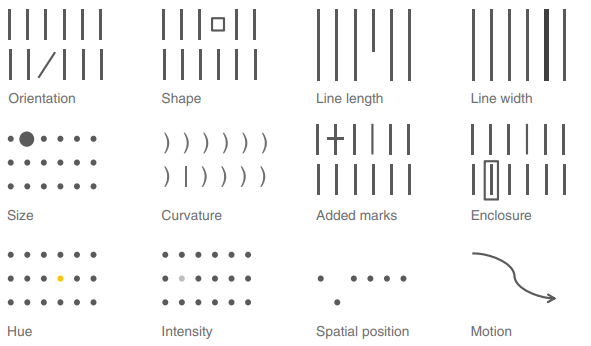
\includegraphics[width=0.8\textwidth]{gfx/preattentive attributes.png}
    \caption{Die präattentiven Attribute von \cite{Knaflic.2016} und \cite{Few.2004}}
    \label{fig:attributes}
    \end{figure}
    Wichtig ist, zu entscheiden, was im Graphen zu den wichtigsten Punkten zählt. Hierzu können etwa folgende Fragen gestellt werden: Welche Aspekte werden sinnvoll hervorgehoben? Was ist eine Ablenkung und kann aus dem Graphen entfernt werden? All diese Punkte sind laut \cite{Knaflic.2016}, \cite{TalksatGoogle.2015} relevant bei dem Bündeln der Aufmerksamkeit des Benutzers.\\
    \item Geschichte erzählen\hfill\\ Im finalen Schritt des Data-Storytellings wird die Geschichte bzw. der Graph logisch aufgebaut. Hierfür müssen ein sinnvoller Anfang und ein Ende festgelegt werden. Zudem soll der Graph ein Fazit und einen Call to Action, also einen Handlungsaufruf, enthalten.
\end{enumerate}
\section{Expertenumfrage mit Auswertung}
Für die fahrzeugspezifischen Daten in der Anwendung sollen in diesem Anwendungsfall auch Trends erkannt werden können, die später mit dem Data-Storytelling angezeigt werden sollen. Da die Trends in den Daten aber spezifisch sind, wurden für das Finden der relevanten Themen in den Daten Experteninterviews durchgeführt. Dabei ist ein Ziel der Befragung, die genauen Punkte, die in den Zeitreihen durch das Data-Storytelling für die Ingenieure hervorgehoben werden sollen, zu definieren und einzugrenzen. Es können insgesamt drei verschiedene Ziele der Umfrage definiert werden:
\begin{enumerate}
    \item Informationen für den ersten Punkt des Data-Storytellings, das Verstehen des Kontextes, sammeln.
    \item Herausfinden, was die relevanten Informationen sind, die in den Graphen dargestellt werden sollen.
    \item Im Falle der Zeitreihen definieren, was es für Trends gibt und wann diese auftreten.
\end{enumerate}
Die Interviews zur Erkennung der Trends werden als qualitative Leitfadeninterviews \cite{Engineering.2018} durchgeführt, um den Experten zu ermöglichen weiter in das Thema einzudringen. Die Experten sind in dem Fall vier Ingenieure, die das Verfahren, mit dem die Daten ausgewertet werden, mitentwickelt haben. Der Leitfaden zu den Interviews sowie Transkriptionen aller Interviews sind in \ref{appendix:interview_trends} zu finden. Die Transkriptionen wurden als vereinfachte Transkription angefertigt, da es für diese Arbeit nicht relevant ist, wie die verschiedenen Sprechweisen der Experten sind. Bei den Experten handelt es sich um Benedikt Mundl \ref{appendix:interview_trends_mundl}, Jeele Böggemann \ref{appendix:interview_trends_boeggemann}, Michael Städele \ref{appendix:interview_trends_staedele} und Florian Zenzinger \ref{appendix:interview_trends_zenzinger}, allesamt Ingenieure mit einer fundierten Erfahrung im Bereich Betriebsfestigkeit von mehr als 45 Jahren. Für das einfachere Prüfen der Textstellen sind im Folgenden die Zeilennummern mit den passenden Textstellen im Anhang verlinkt und durch einen Klick auf die erste Zeilennummer aufrufbar.\\
%line space in nächster Zeile damit die quelle nicht über den fliestext hinausgeht
Um die Interviews wissenschaftlich zu analysieren, wurde MAXQDA\\ \cite{MAXQDA.2023} verwendet und nach den Methoden von \cite{Mayring.2022}, \cite{Kuckartz.2022} und \cite{AndreMorgensternEinenkel.2023} die inhaltlich strukturierende qualitative Inhaltsanalyse erstellt. \\\\Anhand dieser Analyse konnten mehrere Kategorien festgelegt werden, die für das Erkennen der Trends in den Daten von Bedeutung sind. Insbesondere die Kategorien in der Überkategorie Trends sind von Wichtigkeit, da in dieser Kategorie genau die Aussagen zu den Trends erkennbar sind. In der Unterkategorie Aufstiege steigen die Daten über einen Zeitraum an, wie von Michael Städele in den Zeilen \lref{appendix:interview_trends_staedele:aufstiege_1}--390 und \lref{appendix:interview_trends_staedele:aufstiege_2}--449 sowie Benedikt Mundl in den Zeilen \lref{appendix:interview_trends_mundl:aufstiege_1}--116 erläutert wird. Die Kategorie Abstiege ist laut den Interviews weniger relevant, diese wurden nur von Michael Städele in den Zeilen \lref{appendix:interview_trends_staedele:abstiege_1}--390 angesprochen. Die Tatsache, dass die Abstiege nur von einem Experten erwähnt werden, wird später in den Darstellungen von Bedeutung. Bei den Abstiegen handelt es sich um den Gegenpart der Aufstiege, weil die Daten sich hier graduell nach unten entwickeln. Das nächste relevante Element in den Daten sind sogenannte Peaks. Peaks können als Minima oder Maxima in den Daten in Relation zu den umliegenden Werten definiert werden. Laut den Experten Florian Zenzinger (Zeilen \lref{appendix:interview_trends_zenzinger:peaks_1}--599), Michael Städele (Zeilen \lref{appendix:interview_trends_staedele:peaks_1}--449 und Zeilen \lref{appendix:interview_trends_staedele:peaks_2}-473) und Benedikt Mundl (Zeilen \lref{appendix:interview_trends_mundl:peaks_1}--41) werden diese bei der Analyse der Daten als Erstes betrachtet. Rückschließend lässt sich davon ausgehen, dass die Peaks in der Darstellung relevanter sind als beispielsweise die Abstiege. Die nächste Kategorie ist das Offset, auch Drift genannt, hierbei handelt es sich um eine Nullpunktverschiebung in den Daten. Durch das Offset kann beispielsweise eine plastische Verformung am Fahrzeugteil erkannt werden, wie Florian Zenzinger (Zeilen \lref{appendix:interview_trends_zenzinger:offset_1}--730 und \lref{appendix:interview_trends_zenzinger:offset_2}--741), Jeele Böggemann (Zeilen \lref{appendix:interview_trends_boeggemann:offset_1}--352) und Benedikt Mundl (Zeilen  \lref{appendix:interview_trends_mundl:offset_1}--46)  beschreiben. Ein weiteres Datenmuster von Interesse sind Schwingungen, bei denen die Daten zwischen maximalen und minimalen Werten rapide hin und her schwanken. Florian Zenzinger erwähnt Schwingungen in den Zeilen \lref{appendix:interview_trends_zenzinger:schwingungen_1}--678, \lref{appendix:interview_trends_zenzinger:schwingungen_2}--682, \lref{appendix:interview_trends_zenzinger:schwingungen_3}--696, \lref{appendix:interview_trends_zenzinger:schwingungen_4} und \lref{appendix:interview_trends_zenzinger:schwingungen_5}--708, während Michael Städele die Schwingungen in den Zeilen \lref{appendix:interview_trends_staedele:schwingungen_1}--452 beschrieben hat. Ansonsten wurden noch allgemeine Abweichungen beschrieben. Damit sind hauptsächlich Über- oder Unterschreitungen eines bestimmten Wertebereichs gemeint. Diese Abweichungen wurden von Florian Zenzinger in den Zeilen \lref{appendix:interview_trends_zenzinger:abweichungen_1}--607, von Jeele Böggemann in den Zeilen \lref{appendix:interview_trends_boeggemann:abweichungen_1}--246 und \lref{appendix:interview_trends_boeggemann:abweichungen_5}--344 sowie von Benedikt Mundl in den Zeilen \lref{appendix:interview_trends_mundl:abweichungen_1}--134 beschrieben. In Abbildung \ref{fig:trends} werden alle Subkategorien der Trends in visueller Form dargestellt, geordnet nach der Häufigkeit der Erwähnung. 
\begin{figure}[h!]
\centering
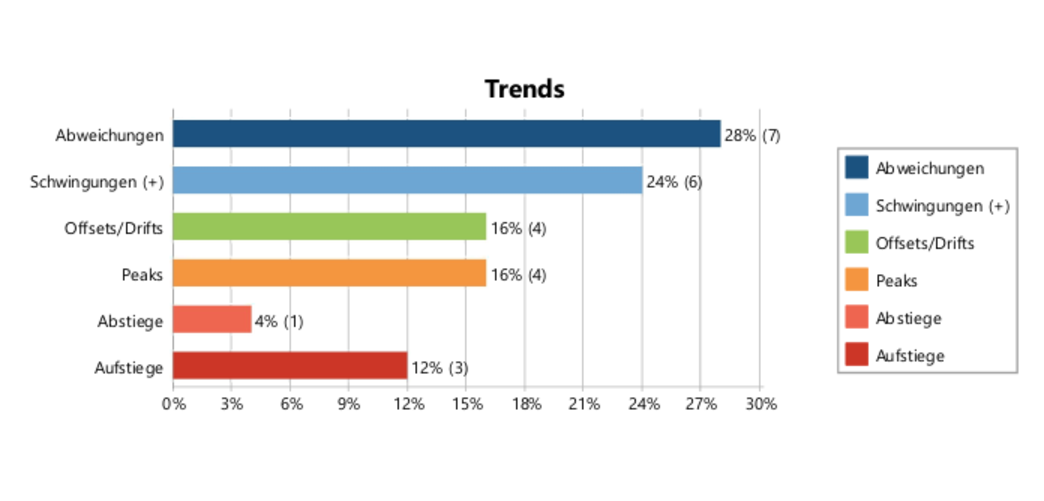
\includegraphics[scale=0.7]{appendix/InterviewTrends/anzahl trends.pdf}
\caption{Die Trendkategorien sortiert nach Häufigkeit der Erwähnung}
\label{fig:trends}
\end{figure}
\\In Bezug auf die Interviews lassen sich auch einige Aussagen zu den Daten allgemein treffen. So wird von Florian Zenzinger in den Zeilen \lref{appendix:interview_trends_zenzinger:daten_1}--717 die Darstellungsmethode \ac{PSD} erklärt. Diese Darstellungsmethode kann laut Herrn Zenzinger bei den Zeitreihen benutzt werden, um die Schwingungen eines Teils darzustellen. Michael Städele (Zeilen \lref{appendix:interview_trends_staedele:daten_1}--431) und Jeele Böggemann (Zeilen \lref{appendix:interview_trends_boeggemann:daten_1}--229, \lref{appendix:interview_trends_boeggemann:daten_2}--270 und \lref{appendix:interview_trends_boeggemann:daten_3}--280) gehen genauer auf die Daten ein, die von den Sensoren geschickt werden. Dabei wird von Michael Städele auch das \ac{DT} erwähnt. Hierbei handelt es sich um das Verfahren, mit dem rechnerisch die Beschleunigungen und Belastungen der Komponenten abgeleitet werden können. Jeele Böggemann erklärt, dass für das Messen \ac{DMS} verwendet werden. In \cite{Keil.2017} wird das Messen mit \ac{DMS} als \glqq [Erfassung der] Dehnungsmessstreifen [von] Dehnungen, die die vom Aufnehmer zu messenden mechanischen Größen im Messkörper des Aufnehmers [hervorrufen]\grqq{}, erklärt. Jeele Böggemann spricht zudem noch von sogenannten Targets, die von Herrn Böggemann als \glqq Wert, mit dem das Fahrzeug abgeprüft wurde\grqq{}, beschrieben werden. In \ref{appendix:general_types} in den Zeilen 51-–73 ist der zum Target passende Datentyp dargestellt.\\\\Zusätzlich zu den allgemeinen Daten werden von den Interviewten auch Aussagen über die Extremwerte und die Schädigungswerte getroffen. Die Extremwerte werden von Florian Zenzinger (Zeilen \lref{appendix:interview_trends_zenzinger:extremwerte_1}--670), von Jeele Böggemann (Zeilen \lref{appendix:interview_trends_boeggemann:extremwerte_1}--235 und \lref{appendix:interview_trends_boeggemann:extremwerte_2}--466) und von Benedikt Mundl (Zeilen \lref{appendix:interview_trends_mundl:extremwerte_1}--27 und \lref{appendix:interview_trends_mundl:extremwerte_2}--176) erwähnt. Sie sind sich einig darüber, dass es sich bei den Extremwerten um die ersten Points of Interest handelt, die sie bei der Analyse prüfen. Daraus resultierend sollen bei der späteren Darstellung von Daten mit dem Data-Storytelling die Extremwerte hervorgehoben werden. Besonders auf \glqq Ausreißer\grqq{} wird bei der Analyse Wert gelegt. Ebenso werden die Schädigungswerte von allen interviewten Personen als wichtig erachtet, von Florian Zenzinger in den Zeilen \lref{appendix:interview_trends_zenzinger:schädigungswerte_1}--677, Michael Städele in den Zeilen \lref{appendix:interview_trends_staedele:schädigungswerte_1}--389 und \lref{appendix:interview_trends_staedele:schädigungswerte_2}--466, Jeele Böggemann in den Zeilen \lref{appendix:interview_trends_boeggemann:schädigungswerte_1}--240 und Benedikt Mundl in den Zeilen \lref{appendix:interview_trends_mundl:schädigungswerte_1}--108, \lref{appendix:interview_trends_mundl:schädigungswerte_2}--110 und \lref{appendix:interview_trends_mundl:schädigungswerte_3}--180. Die Schädigung kann mittels eines Wertes definiert werden, der angibt, wie lange die Lebensdauer eines Bauteils ist.\\
Die Kategorie der Visualisierungen wird in zwei Unterkategorien eingeteilt, die Zeitreihen und die Zählmethoden. Zu den Zählmethoden zählen auch die Erwähnungen von \glqq Kollektiven\grqq{}, vollständig Lastkollektive genannt. Kollektive werden in \cite{Jacobs.2016} definiert als \glqq ein Datensatz, der die Beanspruchung eines Bauteils oder einer Maschine in einem bestimmten Zeitraum abbildet. In einem Lastkollektiv wird der Verlauf der einwirkenden Kraft oder der auftretenden Spannung über [die] Zeit bestimmt\grqq{}. Florian Zenzinger achtet, laut den Zeilen \lref{appendix:interview_trends_zenzinger:zeitreihen_1}--679 und \lref{appendix:interview_trends_zenzinger:zeitreihen_2}--696, in den Zeitreihen besonders auf starke Schwingungen. Indessen wünscht sich Benedikt Mundl laut den Zeilen \lref{appendix:interview_trends_mundl:zeitreihen_1}--190 eine Möglichkeit, mehrere Zeitschriebe miteinander zu vergleichen. Die Zählmethoden werden von Herrn Mundl in den Zeilen \lref{appendix:interview_trends_mundl:zaehlmethoden_1}--186 erwähnt und genauer als Kollektive, Rangepair und Levelcrossing definiert. Laut Jeele Böggemann (Zeilen \lref{appendix:interview_trends_boeggemann:zaehlmethoden_1}--307) ist die Darstellung der Kollektive für ihn besonders relevant. \\\\ Des Weiteren gibt es die Hauptkategorie Plausibilisierung, bei der anhand von automatischer Erkennung direkt überprüft werden sollte, ob die Daten  realistisch und plausibel sind. Die Plausibilisierung allgemein wird von Florian Zenzinger (Zeilen \lref{appendix:interview_trends_zenzinger:plausibilisierung_1}--598) und von Benedikt Mundl (Zeilen \lref{appendix:interview_trends_mundl:plausibilisierung_1}--31) erwähnt. Im Allgemeinen ist bei der Plausibilisierung nur schwierig automatisch zu bestimmen, wann ein Wert realistisch ist, da sich die Ingenieure dabei stark auf ihre Erfahrung verlassen. Aber wenn beispielsweise ein Signal über längere Zeit null ist, obwohl sich das Fahrzeug  bewegt, ist die Wahrscheinlichkeit hoch, dass es sich um einen Defekt oder Messfehler handelt. Hieraus resultiert eine weitere Unterkategorie in der Plausibilisierung: Defekte und Messfehler. Florian Zenzinger (Zeilen \lref{appendix:interview_trends_zenzinger:defekte_1}--616), Michael Städele (Zeilen \lref{appendix:interview_trends_staedele:defekte_1}--445), Jeele Böggemann (Zeilen \lref{appendix:interview_trends_boeggemann:defekte_1}--237) und Benedikt Mundl (Zeilen \lref{appendix:interview_trends_mundl:defekte_1}, \lref{appendix:interview_trends_mundl:defekte_2}--28, \lref{appendix:interview_trends_mundl:defekte_3}--116 und \lref{appendix:interview_trends_mundl:defekte_4}--125) erwähnen allesamt Messfehler oder Defekte an den Sensoren. Solche Fehler erkennt man laut den Interviewten häufig an Peaks, Ausreißern oder an Nullwerten, die von den Sensoren gesendet werden. Auch deswegen sind die Peaks in der Trenderkennung  relevant. Auch bei individuellen Fehlern des Fahrers kann es zu Problemen bei der Plausibilisierung kommen. Jeele Böggemann (Zeilen \lref{appendix:interview_trends_boeggemann:fahrer_1}--274) und Benedikt Mundl (Zeilen \lref{appendix:interview_trends_mundl:fahrer_1}--98 und \lref{appendix:interview_trends_mundl:fahrer_2}--125) sprechen dieses Thema an. Eine Voraussetzung der Messungen ist im Speziellen bei der Dauerlauferprobung ist, die Strecken immer gleich abzufahren. Denn wenn ein Fahrer beispielsweise den Bordstein anfährt oder von der Strecke abkommt, können die Messungen abweichen. Auch hier ist es schwierig, automatisch zu erkennen, wann so ein Fehler vorliegt, da auch das auf der Erfahrung der auswertenden Ingenieure basiert. \\ Zuletzt wurden die interviewten Ingenieure nach den bereits geplanten Unterseiten für die Webseite befragt. Das Dashboard soll laut Florian Zenzinger (Zeilen \lref{appendix:interview_trends_zenzinger:dashboard_1}--659) und Benedikt Mundl (Zeilen \lref{appendix:interview_trends_mundl:dashboard_1}--72) zunächst als Einstieg in die Datenbasis gesehen werden, mit einer Übersicht dazu, welche Einsatzorte und Strecken es in den vorhandenen Daten gibt und welche Fahrzeuge diese abgefahren sind. Zu der Unterseite mit den Vergleichen der Erprobungen und den realen Einsätzen wird von Michael Städele (Zeilen \lref{appendix:interview_trends_staedele:vergleich_1}--551) und Benedikt Mundl (Zeilen \lref{appendix:interview_trends_mundl:vergleich_1}--158 und \lref{appendix:interview_trends_mundl:vergleich_2}-167) angemerkt, dass es sich hier um die wichtigste Unterseite handelt. Der Grund liegt darin, dass durch die Vergleiche berechnet wird, wie ein Fahrzeug voraussichtlich in einem, in der Zukunft liegenden, Einsatz beschädigt wird. Auf der Unterseite der Dauerlauferprobung werden die Daten der Fahrzeuge auf festgelegten Strecken von denselben Fahrern über lange Zeit erprobt. Gleichzeitig werden die Vergleichsdaten gesammelt, die dann auf der Vergleichsseite verwendet werden. Dies wird von Florian Zenzinger (Zeilen \lref{appendix:interview_trends_zenzinger:dauerlauferprobung_1}--646), Michael Städele (Zeilen \lref{appendix:interview_trends_staedele:dauerlauferprobung_1}--511 und \lref{appendix:interview_trends_staedele:dauerlauferprobung_2}--539), Jeele Böggemann (Zeilen \lref{appendix:interview_trends_boeggemann:dauerlauferprobung_1}--299) sowie Benedikt Mundl (Zeilen \lref{appendix:interview_trends_mundl:dauerlauferprobung_1}--80, \lref{appendix:interview_trends_mundl:dauerlauferprobung_2}--105, \lref{appendix:interview_trends_mundl:dauerlauferprobung_3}--108 und \lref{appendix:interview_trends_mundl:dauerlauferprobung_4}--144) übereinstimmend bestätigt. \\\\ Zum Data-Storytelling haben Michael Städele (Zeilen \lref{appendix:interview_trends_staedele:storytelling_1}--402, \lref{appendix:interview_trends_staedele:storytelling_2}--412 und \lref{appendix:interview_trends_staedele:storytelling_3}--557) und Florian Zenzinger (Zeilen \lref{appendix:interview_trends_zenzinger:storytelling_1}--664) einige Ideen für potenzielle Datengeschichten, unter anderem, wo ein Einsatz extrem ist, wie die Bodenbeschaffenheit ist oder wie sich eine Erprobung im Vergleich zu einem tatsächlichen Einsatz verhält. Allgemein zur Entwicklung werden von Jeele Böggemann (Zeilen \lref{appendix:interview_trends_boeggemann:wunsch_1}--316, \lref{appendix:interview_trends_boeggemann:wunsch_2}--329 und \lref{appendix:interview_trends_boeggemann:wunsch_3}--339) und Benedikt Mundl (Zeilen \lref{appendix:interview_trends_mundl:wunsch_1}--199) einige kleinere Wünsche geäußert, eine Funktion zum Sortieren von Balkendiagrammen, vermehrter Einsatz von Hovereffekten zur besseren Einordnung von speziellen Punkten und der Vergleich von Zeitschrieben. Zur besseren Übersicht werden die Ergebnisse der Experteninterviews in Tabelle \ref{2:experteninterview_results} mit einer kurzen Beschreibung und der Häufigkeit der Erwähnungen dargestellt.
\newpage
\label{2:experteninterview_results}
\begin{table}[h!]
\begin{tabular}{p{4cm}|p{6.7cm}|r}
Liste der Kategorien                & Beschreibung                                                                                   & Häufigkeit \\ \hline \hline
Trends                               &                                                                                                &                                \\
\hspace{5mm}Aufstiege                            & Eine graduelle Veränderung der Daten nach oben                                                 & 3                              \\
\hspace{5mm}Abstiege                             & Eine graduelle Veränderung der Daten nach unten                                                & 1                              \\
\hspace{5mm}Extremwerte                                & Ein signifikanter Spitzenwert in den Daten, negativ oder positiv                                                     & 4                              \\
\hspace{5mm}Offset/Drifts                        & Eine Nullpunktverschiebung in den Daten                                                        & 4                              \\
\hspace{5mm}Schwingungen                         & Wiederholte Schwankungen in den Daten                                                          & 6                              \\
\hspace{5mm}Abweichungen                         & Überschreitung der Daten aus dem zuvor festgelegten Wertebereich                                    & 4                            \\ \hline  
Daten                                & Allgemeine Aussagen zu den benutzten Daten                                                      & 5                              \\
\hspace{5mm}Extremwerte                          & Extreme Punkte in den Daten                                                               & 5                              \\
\hspace{5mm}Schädigungswerte                     & Die allgemeine Bezeichnung der Daten, die für die Schädigung einer Komponente berechnet werden  & 7                              \\ \hline  
Visualisierungen                     &                                                                                                &                                \\
\hspace{5mm}Zeitreihen                           & Daten über einen Zeitraum dargestellt                                                   & 3                              \\
\hspace{5mm}Zählmethoden     & In der Mechanik bereits existierende Arten von Darstellungen                                   & 2                              \\  \hline  
Plausibilisierung                    &                                                                                                &                                \\
\hspace{5mm}Defekte/Messfehler               & Defekte oder Messfehler der Sensoren in den Daten                                              & 7                              \\
\hspace{5mm}Fehler des Fahrers                   & Erkennung von individuellen Fehlern beim Fahren, Missuse oder sonstigen Inkonsistenzen                       & 3                              \\    \hline  
Dashboard                            & Aussagen zu der Unterseite Dashboard                                                           & 2                              \\   \hline  
Überwachung Dauerlauferprobung       & Aussagen zu der Unterseite Überwachung Dauerlauferprobung                                      & 8                              \\   \hline  
Vergleiche von Einsatzdaten          & Aussagen zu der Unterseite Vergleiche von Einsatzdaten                                         & 3                              \\\hline  
Data-Storytelling                    & Allgemeine Ideen zum Thema Data-Storytelling und im speziellen Vorschläge für Datengeschichten & 4                              \\\hline  
Wünsche                              & Allgemeine Wünsche für die Darstellungen                                                       & 4                            
\end{tabular}
\centering
\caption {Ergebnisse der Experteninterviews mit Kurzbeschreibungen und Häufigkeiten der Erwähnungen des Themas}
\end{table}

\newpage

\section{Regeln zum Erkennen von Trends in den Zeitreihendaten}
Um die Erkennung der Trends in den Zeitreihen dynamisch ausführen zu können, müssen für jede Art der Erkennung Regeln festgelegt werden, die dann durch die Implementierung die Trends erkennen. Die Implementierung ist in \ref{appendix:trend-detection-code} zu finden und in TypeScript implementiert, um für den Benutzer dynamisch anpassbar zu sein. Thematisch wird die Trenderkennung für Zeitreihen (siehe Datentyp \texttt{TimeSeries} \ref{appendix:graph_types}) implementiert, da diese die Auswirkungen der Kräfte auf verschiedene Komponenten über die Dauer der Messung anzeigen. Die Zeitreihen setzen sich aus dem Nummern-Array \texttt{values} und einer Frequenz, in der die Werte auftreten, zusammen. Die Frequenz wird mit der Anzahl der Werte verrechnet, um die x-Werte zu erzeugen. Die y-Werte bildet der \texttt{values}-Array. Dadurch, dass die Werte der Zeitreihen immer in der gleichen Frequenz auftreten, ist gegeben, dass die einzelnen Datenpunkte stets die gleiche Distanz zueinander haben.
\subsection{Allgemeine Regeln und Funktionen}\label{2:general_implementations}
Für die Berechnungen werden viele Funktionen mehrfach benötigt. Um Code-Wiederholungen zu vermeiden, bessere Lesbarkeit zu ermöglichen und das Testen der Funktionen zu erleichtern, werden hilfreiche Mikrofunktionen erstellt, die in mehreren der Trenderkennungsfunktionen benötigt und genutzt werden. Im Folgenden werden diese kurz erklärt und zusammenfassend dargestellt:
\begin{description}

\item[\texttt{average}] \hfill \\\\
Die Berechnung des arithmetischen Mittels, dargestellt in \ref{appendix:trend-detection-code}[Zeilen 7-–9]. Eine einfache Funktion, die die Datenpunkte annimmt, diese so anpasst, dass alle Werte miteinander addiert werden, und zum Schluss die Summe durch die Anzahl der Werte in dem entsprechenden Array teilt. Die Funktion basiert auf der folgenden mathematischen Formel \ref{eqn:average} aus \cite{Papula.2017}:
\begin{equation}
\label{eqn:average}
         average(x_t)=\frac{x_1+x_2+...+x_n}{n}=\frac{\sum\limits_{i=1}^nx_t}{n} 
\end{equation}

\item[\texttt{getPercentageOfHeight}] \hfill \\\\
Diese Funktion (\ref{appendix:trend-detection-code} Zeilen 18-–22) berechnet den maximalen Wertebereich des Arrays und errechnet anhand einer eingegebenen Prozentzahl die prozentuale Höhe. Hierfür wird der in JavaScript, und somit auch TypeScript, vorhandene Built-in Namespace \texttt{Math} \cite{MDNcontributors.} verwendet, um die maximalen und minimalen Werte des Arrays auszugeben. Dadurch ist die Funktion einfach zu testen und performant. In der folgenden Formel \ref{eqn:height} wird der Rechenweg wiedergegeben, wobei es sich bei der Variable \texttt{p} um die eingegebene Prozentzahl handelt.\\ 
\begin{equation}
\begin{split}
\label{eqn:height}
 height(x_t,p)&=(\max(x_1, x_2, ..., x_n) - \min(x_1, x_2, ..., x_n)) * p \\
&\text{für } \{p \in \mathbb{Q}| 0.01 < p \le 1.00 \}
\end{split}
\end{equation}


\item[\texttt{getPercentageOfDistanceBetweenMarkers}] \hfill \\\\
Ähnlich wie auch bei \texttt{getPercentageOfHeight} wird mit dieser Funktion (\ref{appendix:trend-detection-code} Zeilen 31-–36) berechnet, wie viele Marker wie viel Prozent der gesamten Länge der Zeitreihe entsprechen. Da alle Datenpunkte gleich weit voneinander entfernt sind, lässt sich anhand des Ergebnisses später einfach durch Einsetzen in die Frequenzberechnung erkennen, wo sich die Marker befinden. Daraus bildet sich die mathematische Formel \ref{eqn:distance}.\\
\begin{equation}
\begin{split}
\label{eqn:distance}
    distance(p,n)&= p * n\\ 
    &\text{ wobei }n\text{ der Länge der Zeitreihe entspricht}\\ &\text{ und für }p\text{ gilt }\{p \in \mathbb{Q}| 0.01 < p \le 1.00 \}.\\\
\end{split}
\end{equation}

\item[\texttt{getMovingAverage}]\hfill \\\\
Bei der Funktion \texttt{getMovingAverage} (\ref{appendix:trend-detection-code}, 44-–73) handelt es sich um eine Funktion, die den gleitenden Durchschnitt der Zeitreihe berechnet und diesen als Gleitkommazahlen-Array zurückgibt. Die Funktion ist inspiriert durch das \texttt{optimal solution example} von \cite{RichardBevan.}, wobei die Funktion anhand der mathematischen Formel in \ref{eqn:moving-average} so weit angepasst wurde, dass nur noch die Zeile 56 von der Funktion von \cite{RichardBevan.} vorhanden ist. Der gleitende Durchschnitt ist für die Trenderkennung ein wichtiges Werkzeug \cite{Wiesbaden.2013} und wird von \cite{Hyndman.2011} definiert als Zeitreihe, die aus mehreren Durchschnitten von mehreren aufeinanderfolgenden Werten einer anderen Zeitreihe gebildet wird. Für die Berechnung wird ein \texttt{window} festgelegt, das die Anzahl der Werte festlegt, die für die Durchschnittsberechnung einbezogen werden sollen. Das bedeutet allerdings auch, dass somit die Durchschnittswerte für den Anfang und das Ende der Zeitreihe nicht berechnet werden können. Aus diesen Gründen wurden die Zeilen 48–-56 und 65-–71 ergänzt. Dabei wird für den Anfangs- und Endbereich jeweils eine gleitende Durchschnittsberechnung ausgeführt, die nur in die jeweilige Richtung, die vorhanden ist, berechnet, anstatt das \texttt{window} in beide Richtungen vom Ausgangswert zu verschieben. Dadurch wird das Ergebnis-Array gefüllt, damit später die Anzahlen des Ergebnisarrays und des Arrays der tatsächlichen Zeitreihe miteinander übereinstimmen. Das ist wichtig, da auch die Frequenz, in der die Werte auftreten, übereinstimmen muss, damit beispielsweise beim Bilden der Auf- und Abstiege die richtigen Positionen angegeben werden.  Da sich das \texttt{window} dynamisch aus der Anzahl der Punkte der tatsächlichen Zeitreihe und einem festen Wert bildet, wurde die Zeile 45 ergänzt, um Rechenfehler zu vermeiden. Mit der Standardfunktion \texttt{toFixed()} wird eine Zahl in einen String umgewandelt und dabei wird die Länge der Dezimalstellen auf null begrenzt. Das + vor \texttt{window.toFixed()} wandelt den String automatisch wieder in eine Zahl um. In Abbildung \ref{fig:movingAverage} wird eine Zeitreihe mit dem gleitenden Durchschnitt berechnet, durch die Funktion mit einem \texttt{window} von der Länge des Arrays geteilt, durch den Faktor 50 dargestellt. Da die Zeitreihen variable Längen haben, soll, weil das \texttt{window} dadurch von der Länge der Zeitreihe abhängt, gewährleistet werden, dass der gleitende Durchschnitt sich verhältnismäßig bei allen Zeitreihen gleich verhält. 

\begin{figure}[h!]
\centering
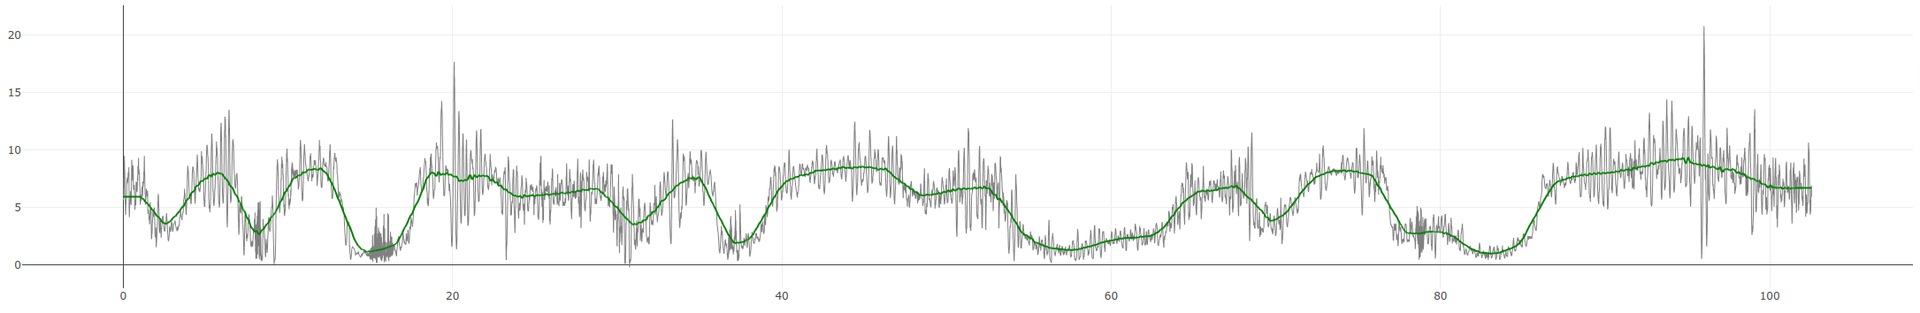
\includegraphics[width=\textwidth]{gfx/movingAverage.png}
\caption{Gleitender Durchschnitt}
\label{fig:movingAverage}
\end{figure}
Mathematisch wird der gleitende Durchschnitt ungerader Ordnung von \cite{Bosch.2002} definiert als:
\begin{equation}
\label{eqn:moving-average}
    \begin{split}
        movingAverage(x_t,m)&=\frac{1}{2m+1}(x_{t-m}+x_{t-m+1}+...+x_t+...+x_{t+m})\\
&=\frac{1}{2m+1}\sum\limits_{j=-m}^mx_{t+j} \text{ mit }\{m\in \mathbb{N}\}\\
    \end{split}
\end{equation}
Dabei steht $m$ für das \texttt{window}, das für den gleitenden Durchschnitt festgelegt wurde, und $x_t$ für die Zeitreihe.
Da bei der Erstellung des gleitenden Durchschnitts ungerader Ordnung jeweils am Anfang und am Ende der Zeitreihe \[k=\frac{m}{2}\] herausfallen, werden diese Werte bei der Implementation am Anfang der Zeitreihe mit \[\frac{1}{m+1}(x_{t}+x_{t+1}+...+x_{t+m})\] und am Ende der Zeitreihe mit  \[\frac{1}{m+1}(x_{t-m}+x_{t-m+1}+...+x_t)\] ergänzt. \\\\

\item[\texttt{findLocalExtreme}]\hfill \\\\
Die Funktion (\ref{appendix:trend-detection-code} Zeilen 81-–99) findet lokale Minima und lokale Maxima der Zeitreihe und gibt diese aus. Die Funktion basiert auf der Implementation von \cite{SamuelProll.2022} und wurde hier so weit abgeändert, dass damit nicht nur Maxima, sondern auch Minima gefunden werden können (Zeilen 86, 91–-97). Es wurde eine boolesche Variable \texttt{findMaxima} hinzugefügt, die zwischen der Suche nach Minima und Maxima unterscheidet. Die Funktion iteriert durch alle Punkte des Wert-Arrays und vergleicht die direkten Nachbarn mit dem aktuellen Punkt. Bei den Maxima müssen der linke und rechte Nachbar jeweils niedriger sein als der aktuelle Punkt. Bei den Minima ist diese Bedingung genau umgekehrt, beide Nachbarn müssen also höher sein als der aktuelle Punkt. In der folgenden Formel \ref{eqn:minmax} werden die Bedingungen mathematisch formuliert.
\begin{equation}
\label{eqn:minmax}
    \begin{split}
        &\text{Im Folgenden steht }x_t\text{ für die Zeitreihe und }n\text{ für die Länge dieser.}\\
       & \text{Wenn Maxima gesucht werden:}\\&
        	Maxima(x_t, n)=\{ x_i \in {1, 2, ..., n}| x_i > x_{i-1} \wedge x_i > x_{i+1}\}\\
         & \text{Wenn Minima gesucht werden:}\\&
        	Minima(x_t, n)=\{ x_i \in {1, 2, ..., n}| x_i < x_{i-1} \wedge x_i < x_{i+1}\}\\
    \end{split}
\end{equation}
\end{description}

\subsection{Aufstiege und Abstiege}
\label{subsection:risesAndFalls}
Die Berechnungen für die Auf- und Abstiege funktionieren ähnlich zueinander. Der entsprechende Code ist in \ref{appendix:trend-detection-code:aufstiege} zu sehen. Zur Vermeidung von Wiederholungen wird nur die Funktion für die Aufstiege erklärt, da die Funktion für die Abstiege sich allein durch die Bedingungen in den If-Abfragen unterscheidet. Für die Funktion werden ausschließlich die y-Werte benötigt. Die Funktion kann aber, falls gewünscht (für das Data-Storytelling), mit Benutzereingaben erweitert werden. Aus Performancegründen wird ebenso der gleitende Durchschnitt als Variable in die Funktion mit übergeben, da der gleitende Durchschnitt von mehreren Funktionen der Trenderkennung genutzt wird und so nur einmal berechnet werden muss. Die Funktion liefert einen Array aus Anfangs- und Endpunkten der Anstiege. Wichtig für die Erkennung der Aufstiege sind folgende Variablen, die auch durch den Nutzer manuell eingegeben werden können:
\begin{itemize}
    \item Minimale Distanz zwischen dem Start- und Endpunkt in Prozent, um die minimale Länge eines Anstiegs/Abstiegs festzulegen
    \item Minimale Höhe zwischen den Start- und Endwerten in Prozent
\end{itemize}
Grundlegend funktioniert die Berechnung so: Der gleitende Durchschnitt wird Punkt für Punkt durchgegangen und jeder Punkt wird mit seinen Nachbarn verglichen. Befindet sich der Punkt in einem Anstieg, ist sein linker Nachbar niedriger und sein rechter Nachbar höher, wird der Punkt übersprungen. Ist der Punkt der Anfang eines Anstiegs, also der linke Nachbar höher oder gleich hoch und der rechte Nachbar ebenso höher ist, wird der Punkt als Startpunkt angesehen. Es kann nur ein Endpunkt erkannt werden, wenn bereits ein definierter Startpunkt gefunden wurde und wenn der aktuelle Punkt höher als der linke Nachbar ist und niedriger oder gleich hoch wie der rechte. Wenn ein definierter Startpunkt und ein definierter Endpunkt existieren, diese Punkte auch im Array der \texttt{values} vorhanden sind, also bei der Erstellung des gleitenden Durchschnitts keine Fehler aufgetreten sind, dann kann geprüft werden, ob der Anstieg durch die minimale Distanz und die minimale Höhe auch als Anstieg zugelassen werden soll. Nachdem geprüft worden ist, ob ein Start- und Endpunkt als Anstieg zählen, und diese ggf. in das Ergebnisarray \glqq gepusht\grqq{} worden sind, werden der aktuelle Start- und Endpunkt entfernt, damit der nächste Anstieg erkannt werden kann.
Die Abstiegsfunktion unterscheidet sich durch die Bedingungen, unter denen ein Start- oder Endpunkt erkannt wird. Diese sind genau gegensätzlich zu den Anstiegen. In Abbildung \ref{fig:risesAndFalls} werden sowohl die Anstiege als auch die Abstiege und der gleitende Durchschnitt, erkannt durch den beschriebenen Code, dargestellt. Für die Variablen wurde bei An- und Abstiegen als minimale Distanz zwischen den Punkten 1 \% und als minimale Höhe 20 \% angegeben. 
\begin{figure}[h!]
\centering
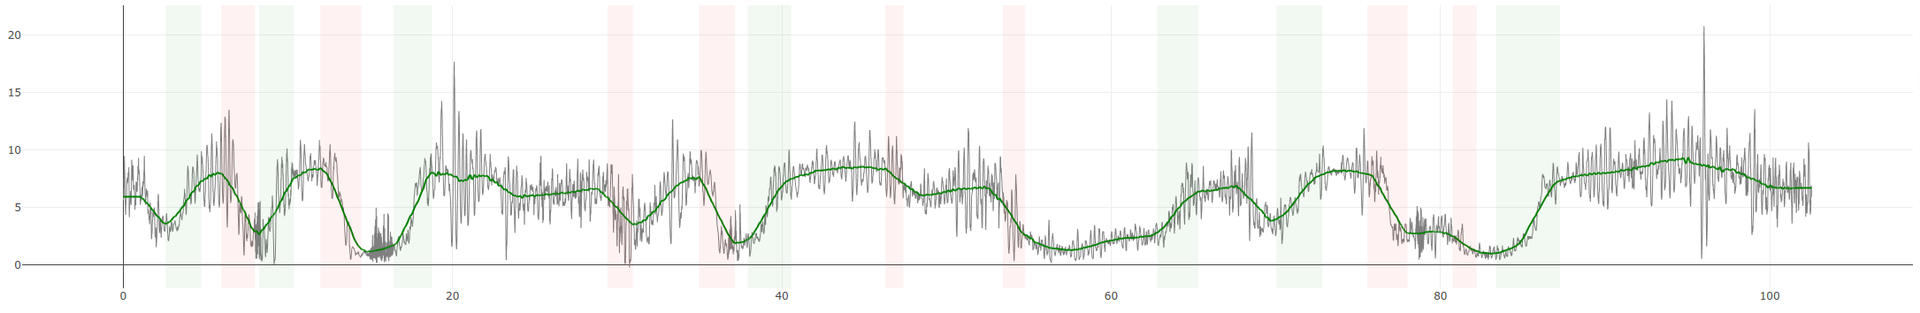
\includegraphics[width=\textwidth]{gfx/falls_rises_movingAverage.png}
\caption{Aufstiege und Abstiege mit gleitendem Durchschnitt}
\label{fig:risesAndFalls}
\end{figure}

\subsection{Extremwerte}
Die Funktion zum Erkennen der Extremwerte (\ref{appendix:trend-detection-code:peaks}) basiert auf \cite{SamuelProll.2022}, der Funktionalitäten von SciPy zum Finden von Peaks in JavaScript konvertiert hat. SciPy ist eine Ansammlung von mathematischen Algorithmen basierend auf NumPy \cite{TheSciPycommunity.2023}, wobei NumPy eine Python Library ist, die auf Simulationswissenschaften spezialisiert ist \cite{NumPyDevelopers.2022}. Ebenso wurde in der Erkennung eine Funktion für einen \texttt{argsort} benötigt, diese basiert auf \cite{EranW.2020}, da es in JavaScript keinen nativen \texttt{argsort} gibt. Ähnlich zu den Aufstiegen und Abstiegen kann auch bei den Extremwerten durch verschiedene Variablen beeinflusst werden, wie präzise die Erkennung ist. Dazu gibt es die folgenden Variablen, alle in Prozent angegeben:
\begin{itemize}
    \item Minimale Höhe von Maxima 
    \item Maximale Höhe von Minima
    \item Distanz zwischen den einzelnen Werten
    \item Puffer zum gleitenden Durchschnitt
\end{itemize}
Die Funktion \texttt{detectExtremesInData} (222--276) startet die Erkennung von Minima und Maxima und berechnet die vom Benutzer eingegebenen Parameter. Dazu werden die Hilfsfunktionen in \ref{2:general_implementations} genutzt. Danach wird die Berechnung an die Funktion \texttt{findExtremes} weitergeleitet. \texttt{findExtremes} ruft zuerst die Funktion \texttt{findLocalExtreme} auf, um die Extremwerte zu bestimmen. Anschließend werden die Werte anhand der oben genannten Variablen gefiltert. Hierbei kann auch komplett auf die Filter verzichtet werden, da diese optional sind. Als Erstes wird nach der Höhe der Werte gefiltert (Zeilen 32–-41). Dazu wird die Built-in-Funktion \texttt{Array.prototype.filter()} verwendet. Es wird unterschieden, ob Minima oder Maxima gefunden werden sollen, und anhand dessen unter oder über der Höhe gefiltert. Um die Funktion auch bei Zeitreihen einzusetzen, die negative Werte erreichen, muss die berechnete Höhe von dem kleinsten Wert der Zeitreihe abgezogen werden. Mathematisch lässt sich diese Funktion folgendermaßen definieren \ref{eqn:filterMinMax}:
\begin{equation}
\label{eqn:filterMinMax}
\begin{split}
   & \text{Filtern der Höhe von Maxima}\\
    &filterByHeight(extremes, x_t, height) = \{x_i \in extremes|x_i>(min(x_t)+height)\}\\
   &\text{Filtern der Höhe von Minima}\\
   & filterByHeight(extremes, x_t, height) = \{x_i \in extremes|x_i<(min(x_t)+height)\}\\
   \\
    \end{split}
\end{equation}
Als Nächstes wird nach Distanz gefiltert, diese Funktion basiert auf \cite{SamuelProll.2022}, wobei die Funktion für das Filtern nach Minima in den Zeilen 59–-62 ergänzt wurde. Bei der Funktionsweise ist wichtig zu erwähnen, dass die Funktion nicht nur nach der Distanz der Werte filtert, sondern dabei auch berücksichtigt, welcher Extremwert höher (oder tiefer) ist, und sich dann je nachdem für den höheren (oder tieferen) Extremwert entscheidet. Die Funktion von \cite{SamuelProll.2022} unterscheidet sich laut dem Autor nur leicht von der SciPy-Implementation und wurde hauptsächlich davon übernommen. Zunächst werden die bereits gefundenen und über die Höhe gefilterten Indices der Extremwerte auf ihre tatsächlichen Höhen gemappt. Danach wird durch die Funktionen von \cite{EranW.2020} der \texttt{argsort} durchgeführt. Laut \cite{NumPyDevelopers.2024} gibt eine \texttt{argsort}-Funktion die Indices aus, wie sie sortiert würden. Um die Funktionen auch für negative Werte in der Zeitreihe zu optimieren, wurde Zeile 23 im Code erweitert. Die native JavaScript-\texttt{sort()}-Funktion sortiert Werte lexikografisch \cite{MDNcontributors.2024}. Das funktioniert in gewisser Weise auch mit Zahlen, da diese einfach zu Strings konvertiert werden. Werden die Zahlen allerdings komplexer oder auch nur negativ, muss in der \texttt{sort()}-Funktion explizit definiert werden, wie sortiert werden soll. Je nachdem, ob Minima oder Maxima gesucht werden, wird danach die Reihenfolge der sortierten Höhen umgedreht. Dann wird im Code in der Reihenfolge der Höhe analysiert, wie weit die Nachbar-Extremwerte vom aktuellen Extremwert entfernt sind, und je nachdem werden die ggf. überflüssigen Extremwerte aus dem Ergebnis entfernt. Dadurch werden automatisch die höchsten Werte behalten, da diese die ersten sind, die verglichen werden.\\\\Zuletzt werden die übrigen Extremwerte über den gleitenden Durchschnitt gefiltert. Diese Funktionalität wurde zu den Funktionen von \cite{SamuelProll.2022} ergänzt. Anhand des eingegebenen Puffers werden nur die Extremwerte übernommen, die einen definierten Abstand vom gleitenden Durchschnitt überschreiten. Hierfür wird der Wert des aktuellen Extremwertes mit dem gleitenden Durchschnitt an der gleichen Stelle verglichen, abzüglich oder zuzüglich (je nachdem, ob Minima oder Maxima gefunden werden sollen) des Puffers. Dabei lautet die mathematische Notation dieser Bedingungen wie in Formel \ref{eqn:filterMovingAverage} dargestellt.
\begin{equation}
\label{eqn:filterMovingAverage}
    \begin{split}
        &\text{Filtern mit dem gleitenden Durchschnitt von Maxima}\\
        &filterMA(extremes,x_t,mA_t, buffer) = \{i \in extremes|x_i>(mA_i+buffer)\}\\
        &\text{Filtern mit dem gleitenden Durchschnitt von Minima}\\
        &filterMA(extremes,x_t,mA_t, buffer) = \{i \in extremes|x_i<(mA_i-buffer)\}
        \\\\
    \end{split}
\end{equation}
In Abbildung \ref{fig:peaks} wird die Extremwerterkennung für Minima und Maxima durchgeführt. Als Variablen wurden für die minimale Höhe der Maxima 75 \%, für die maximale Höhe der Minima 25 \%, als Distanz zwischen den Werten 2 \% und als Puffer 20 \% angegeben. Besonders bei den Minima ist zu sehen, dass die Filterung durch den gleitenden Durchschnitt unbedingt nötig ist, da sich ein Großteil des Signals unter 25 \% Höhe befindet. Für die bessere Erkennbarkeit der Peaks wird in Abbildung \ref{fig:peaks} nur ein Teil der Zeitreihe dargestellt.
\begin{figure}[h!]
\centering
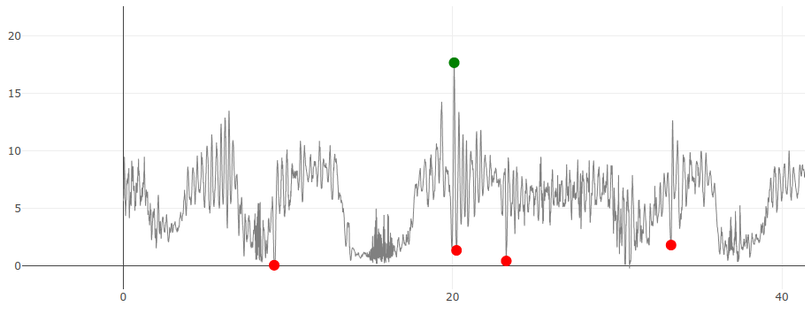
\includegraphics[width=\textwidth]{gfx/peaks.png}
\caption{Maxima und Minima}
\label{fig:peaks}
\end{figure}


\subsection{Offsets und Drifts}
Wie in den Interviews (Kapitel \ref{2:experteninterview_results}) erklärt wird, handelt es sich bei Offsets und Drifts um ein Phänomen, das auftritt, wenn Bauteile plastisch verformt werden. Von den Experten wird bestätigt, dass das Offset und auch Drifts dann erkennbar werden, wenn der Durchschnittswert am Anfang und der Durchschnittswert am Ende eines Graphen drastisch divergieren. Offset und Drift unterscheiden sich durch die Art der Veränderung am Durchschnittswert. Bei Drifts handelt es sich um eine Verschiebung über die Zeit, bei Offsets ist die Verschiebung eher ruckartig. In der Implementation der Funktion zur Erkennung des Offsets in \ref{appendix:trend-detection-code:offsets} lässt sich in den Zeilen 2 und 3 erkennen, dass die gelieferten Daten jeweils in eine vordere Hälfte und eine hintere Hälfte eingeteilt werden und danach die allgemeine Funktion zum Berechnen des Durchschnitts (siehe \texttt{average} \ref{2:general_implementations}) aufgerufen wird. Hierzu wird die \texttt{Array.prototype.slice()}-Funktion von klassischem JavaScript verwendet \cite{MDNcontributors.2020}. In Zeile 6 wird der Pufferwert rechnerisch bestimmt, der gemeinsam mit dem Durchschnittswert des ersten Arrays überschritten  sein muss, um die Offset-Warnung bei kleinen Unterscheidungen zu vermeiden. Schließlich tritt das Offset nur bei drastischen Unterschieden auf. Der Pufferwert wird durch eine Erhöhung von 10\,\% und die allgemeine Funktion von \texttt{getPercentageOfHeight} aus \ref{2:general_implementations} festgelegt. Wenn die Graphen später mit Data-Storytelling überarbeitet werden, lässt sich dieser hart codierte Wert noch durch eine Benutzereingabe ersetzen. Abschließend wird geprüft, ob die Summe des Durchschnitts der ersten Hälfte und des Pufferwerts kleiner ist als die Summe des Durchschnitts der zweiten Hälfte (Zeile 7). Wenn dies zutrifft, wird eine plotly.js-Annotation von der Funktion zurückgegeben, die als Fehlermeldung abgebildet wird.

\subsection{Schwingungen}
Sollten Minima und Maxima direkt aufeinanderfolgen, wird das in dieser Arbeit als Schwingung definiert. Die passende Funktion zu der Schwingungserkennung ist in \ref{appendix:trend-detection-code:schwingungen} nachzuvollziehen. Auch die Schwingungserkennung ist durch Eingaben anpassbar:
\begin{itemize}
    \item Höhe zwischen Minima und Maxima
    \item Distanz zwischen Minima und Maxima
\end{itemize}
Da die Extremwerte bereits mit der \texttt{findLocalExtreme}-Funktion erkannt werden, hat diese Funktion hauptsächlich den Zweck, Minima und Maxima zu vergleichen und zu prüfen, ob sie den eingegebenen Variablen entsprechen. Dazu wird zuerst die Reihenfolge des Auftretens dahingehend geprüft, ob der Maximalwert oder der Minimalwert zuerst eintritt. Aufgrund dieser Prüfung kann je nachdem, welcher Wert zuerst kommt, bestimmt werden, ob die Distanz zwischen den Extremwerten die eingegebene Distanz übersteigt. Wenn dies zutrifft, wird die Höhe der Schwingung geprüft. Wenn beide Bedingungen, also die Höhe der Schwingung und die Distanz zwischen den Extremwerten, erfüllt sind, wird die Kombination aus Maxima und Minima als Schwingung zurückgegeben. In Abbildung \ref{fig:vibrations} wurden die Schwingungen mit einer Distanz von 1\,\% und einer Höhe von 30\,\% festgelegt. 
\begin{figure}[h!]
\centering
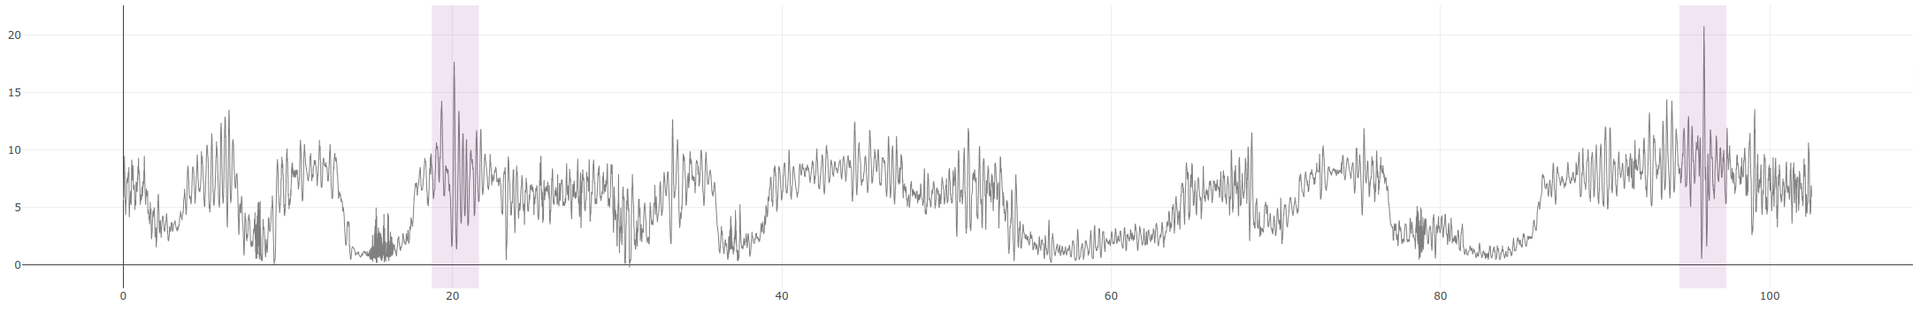
\includegraphics[width=\textwidth]{gfx/vibrations.png}
\caption{Schwingungen}
\label{fig:vibrations}
\end{figure}

\subsection{Abweichungen}
Eine Abweichung wurde von den Experten (siehe Kapitel \ref{2:experteninterview_results}) als Ausbruch aus einem gewissen Wertebereich beschrieben. Hierfür kann der Benutzer entweder einen speziellen Wertebereich für die Markierungen eingeben oder die Funktion in \ref{appendix:trend-detection-code:abweichungen} kann durch die Eingabe eines Puffers einen Wertebereich berechnen, der sich am Durchschnitt aller y-Werte orientiert. Sollte der Benutzer keinen Puffer eingegeben haben, wird mit einem Defaultwert von 20\,\% Puffer gerechnet. Dazu wird mit der allgemeinen \texttt{average}-Funktion der gesamte Durchschnitt ermittelt und dann der Puffer addiert, um die obere Grenze des Wertebereichs, bzw. der Puffer subtrahiert, um die untere Grenze des Wertebereichs zu berechnen. In Abbildung \ref{fig:deviations} werden die Grenzen des Wertebereichs mit 20\,\% Puffer abgebildet. Aus Gründen der besseren Erkennbarkeit wird nur ein Teil der Zeitreihe in \ref{fig:deviations} dargestellt.
\begin{figure}[h!]
\centering
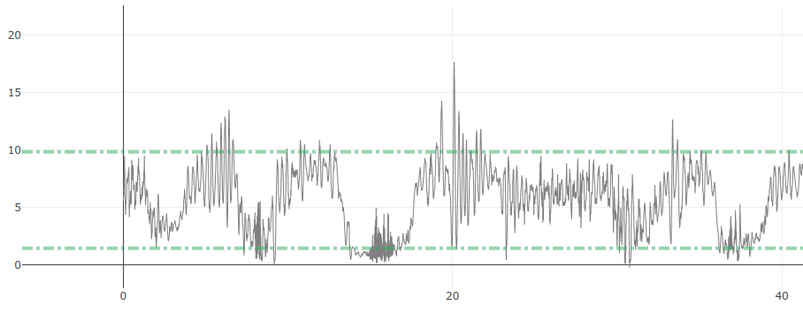
\includegraphics[width=\textwidth]{gfx/deviations.png}
\caption{Abweichungen}
\label{fig:deviations}
\end{figure}
\section{Anwendung des Data-Storytelling}
Im Folgenden werden die Methoden aus \ref{sec:methoden} auf die tatsächlichen Graphen angewandt und implementiert.
\subsection{Prozentuale Schädigung zum groben Überblick}\label{section:Prozentuale_Schädigung}
Grundlegend wird die Datenbasis genutzt, um einen kurzen Überblick über die gesamte Datenlage zu bekommen. Auf der Datenbasis soll ein Graph mit Data-Storytelling entwickelt werden. Wählt man über die Fahrzeugkarten ein einzelnes Fahrzeug aus, soll das kumulierte Lastgeschehen der bewerteten Baugruppen dargestellt werden. \\\\
1. Kontext verstehen:\\
Wie von \cite{Knaflic.2016} empfohlen, wird zunächst Storyboarding mit Stift und Papier betrieben, um einen generellen Entwurf für den Graphen anzufertigen. Danach wird das Tool Figma \cite{FigmaGmbH.2024} genutzt, um einen groben Entwurf zu erstellen. Dieser grobe Entwurf ist in Abbildung \ref{fig:datenbasis} dargestellt.

\begin{figure}[h!]
\centering
\fbox{
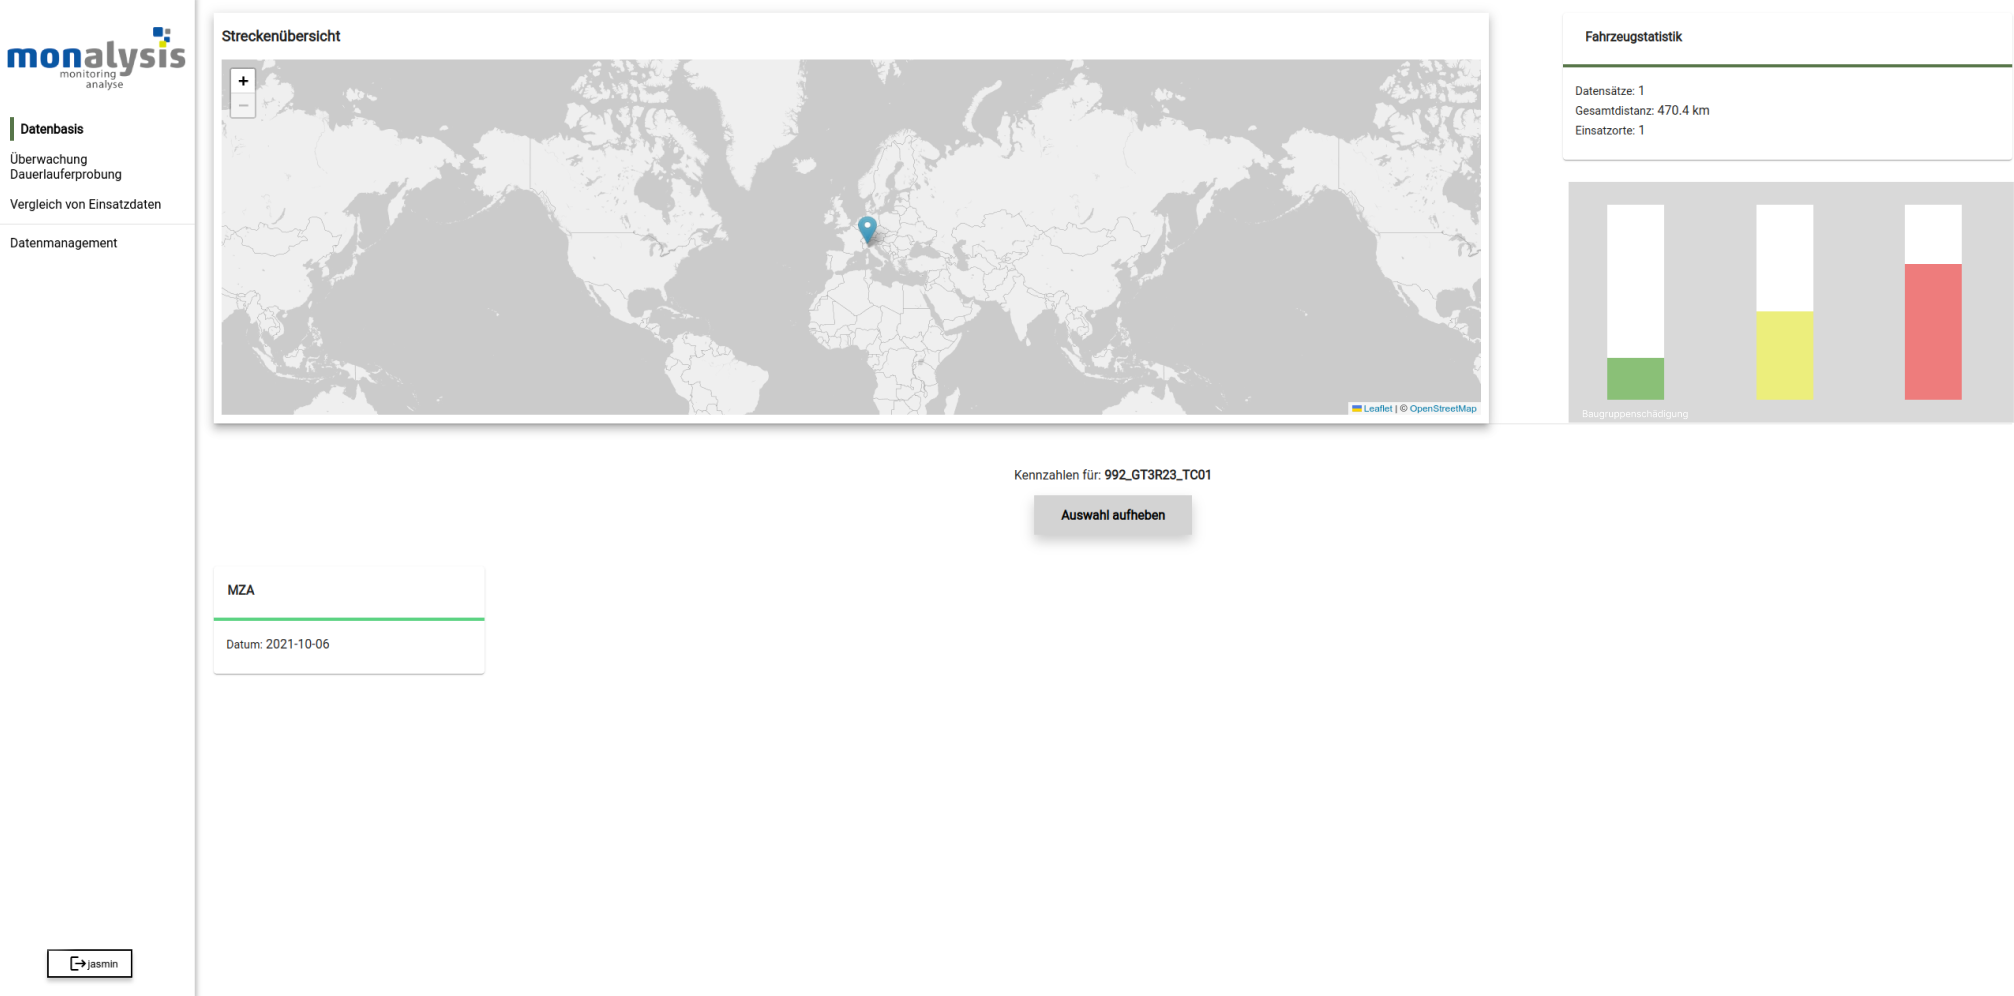
\includegraphics[width=0.8\textwidth]{gfx/Figma_Datenbasis.png}}
\caption{Figma-Entwurf für die Fahrzeugdarstellung der Datenbasis}
\label{fig:datenbasis}
\end{figure}
Die bewerteten Baugruppen werden pro Fahrzeug festgelegt als:
\begin{multicols}{2}
\begin{itemize}
    \item Gesamtfahrzeug
    \item Feder-Dämpfer-System Vorderachse
    \item Feder-Dämpfer-System Hinterachse
    \item Querlenker Vorderachse
    \item Querlenker Hinterachse
    \item Spurstange
    \item Lenkgetriebe
\end{itemize}
\end{multicols}
\noindent
Pro Baugruppe gibt es durch die Erprobung einen Grenzwert, ab dem die Baugruppe kritisch wird. Deshalb ist es sinnvoll, das Lastgeschehen als Prozentwert zu dem Grenzwert darzustellen. Bei der Zielgruppe dieses Graphen handelt es sich, wie bei allen Graphen, um Ingenieure, Maschinenbauer und Fahrzeugbauer. \\\\
2. Darstellung wählen:\\
Bei dieser Darstellung ist die Hauptinformation, wie das Lastgeschehen der einzelnen Baugruppen im Vergleich zu den erprobten Werten ist. Aus diesem Grund würden sich Gauge-Charts oder Bullet-Charts besonders gut eignen. Eine Gauge-Chart wird laut \cite{Schwabish.2021} typischerweise in einem Kreis oder Halbkreis dargestellt, dabei wird eine \glqq Nadel\grqq{} oder auch ein Pointer genutzt, um den aktuellen Wert auf einer Skala anzuzeigen. \cite{Schwabish.2021} beschreibt die Gauge-Chart als einen Graphen, der sich dazu eignet, eine generelle Auskunft über die Datenlage zu geben. Für mehr Details sollte aber eine andere Darstellungsart gewählt werden. Da bei dem aktuellen Fall relativ viele Baugruppenzustände dargestellt werden sollen und eine einzelne Gauge-Chart durch die runde Form zu viel Platz in Anspruch nimmt, sollte bei diesem Graphen eher eine Bullet-Chart gewählt werden. Bullet-Charts sind eine Weiterentwicklung der Gauge-Chart \cite{Schwabish.2021}. Generell sind Bullet-Charts lineare Versionen der radialen Gauge-Chart. Da die Bullet-Chart kompakt ist, eignet sie sich gut dafür, mehrere Werte übereinander darzustellen. \\\\
3. Ordnung schaffen:\\
Basierend auf dem Beispiel für eine Bullet-Chart von \cite{Plotly.2024c} wird zuerst eine Grundlage für die neue Chart geschaffen. Diese ist in Abbildung \ref{fig:bullet_chart_after} zu sehen.
Beim Ordnungschaffen geht es darum, nicht zwingend notwendige Bestandteile des Graphen zu entfernen. Zunächst wird das Delta unter den Zahlwerten entfernt, das Delta zeigt die Veränderung der Werte im Vergleich zu anderen Zeitpunkten. Bei diesem Usecase ist es aber kaum möglich, dass die Schädigung der Bauteile fällt, außer es werden Bauteile ausgetauscht, was die Schädigung dann aber auf den Wert null resetten würde. Es bietet sich auch an, den White Space zwischen den einzelnen Bullets zu erhöhen, um eine bessere Lesbarkeit der Legende zu erreichen. Eine weitere Möglichkeit wäre, eine Legende auf die gesamten Bullets zu beziehen, da die Werte in Prozent dargestellt werden sollen und dadurch immer den gleichen Wertebereich haben. Dadurch würde auch der Visual Clutter reduziert. Zudem wäre es möglich, die Werte, die \glqq zusammengehören\grqq{}, wie Querlenker Vorderachse und Querlenker Hinterachse, durch das Gestalt-Principle  \cite{Schwabish.2021} Connection, also Verbindungen, zu gruppieren. Die Schädigung soll in Prozent dargestellt werden, also bietet es sich auch an, beide Werte in einer gemeinsamen Bullet-Chart zusammenzufassen, da die beiden Querlenker auch dieselben Kriterien dafür haben, wann ein Prozentwert kritisch ist. Die Markierung für den Threshold kann ebenso entfernt werden. Auch die Nummer neben den Bullets kann entfernt werden, da es bei dieser Darstellung nicht um den genauen Wert geht, sondern eher um einen Überblick, wie es um das Fahrzeug steht. Deswegen können auch die Ticks entfernt werden. Mit den oben beschriebenen Änderungen kann der Graph auf Abbildung \ref{fig:bullet_chart_after} reduziert werden.\\\\
\begin{figure}
\centering
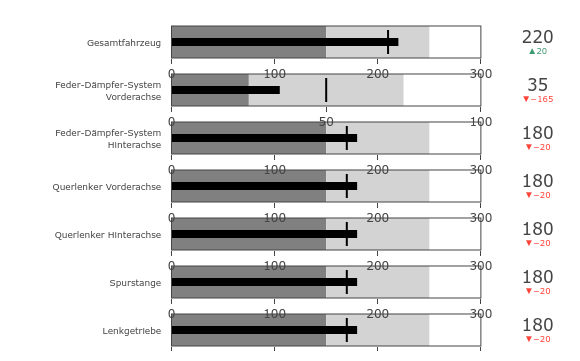
\includegraphics[width=.45\textwidth]{gfx/Bullet_Chart_Before.png} % Just stack two includegraphics!
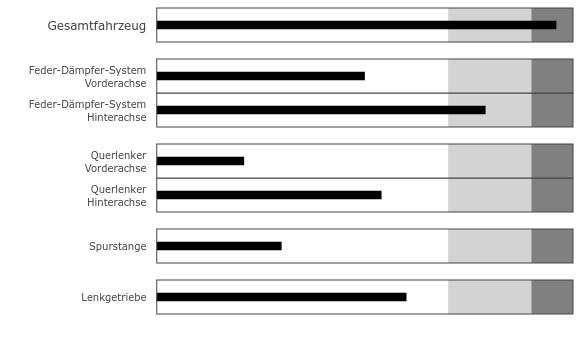
\includegraphics[width=.45\textwidth]{gfx/Bullet_Chart_After.png}
\caption{Bullet-Chart vor und nach dem Ordnungschaffen}
\label{fig:bullet_chart_after}
\end{figure}
4. Aufmerksamkeit bündeln:\\
Die Aufmerksamkeit des Benutzers soll bei dieser Darstellung auf die Bauteile gelenkt werden, die sich nah an den warnenden Zonen bei 70\,\% oder sogar an den kritischen Zonen der Schädigung der Bauteile bei 90\,\% befinden. Es bietet sich an, die bislang in verschiedenen Grautönen gehaltenen Steps je nach Status einzufärben. Als Farben wird für die kritischen Bereiche ein Pastellrot und für die Warnungsbereiche ein Pastellorange gewählt, für die nicht kritischen Bereiche ein Pastellgrün, um so bei dem Benutzer die Assoziation mit einer Ampel auszulösen. Da es sich bei den Benutzern um Ingenieure und Maschinenbauer handelt, ist davon auszugehen, dass diese Assoziation vom Gehirn schnell erzeugt werden kann. Bei den Farben wird darauf geachtet, dass diese auch auf einer Grauskala gut erkennbar sind. Auch der Wert des Gesamtfahrzeugs sollte herausstechen, dafür wird die Schriftgröße des Labels angepasst. Die Farbe des Values wird bei den anderen Gauges zu einem dunklen Grau angepasst.\\\\
5. Geschichte erzählen:\\
Als logischer Call to Action ergibt sich aus dem Graphen der Aufruf zur Wartung eines Fahrzeugs, falls Werte die pastellroten Bereiche des Graphen erreichen sollten, da nach der Schädigung im Ausmaß von 100\,\% nicht mehr davon ausgegangen werden kann, dass das Fahrzeugteil weiter einsatzfähig ist. Da sich der Graph im Layout der Seite eher im Hintergrund befindet, ist es empfehlenswert, diese wichtige Warnung an anderer Stelle einzublenden. Dafür eignet sich eine Position direkt unter der Karte, damit die Warnung in das Auge fällt. Die gewählte Aufteilung des Graphen ist zufälligerweise bereits in den vorherigen Graphen vorhanden. Das Gesamtfahrzeug sollte an erster Stelle stehen, da es sich bei dem Wert um die Summe aller anderen Werte handelt. Zudem wird ein dezenter Strich als Trennung des Gesamtfahrzeugs von den Werten der Fahrzeugkomponenten eingefügt, um zu verdeutlichen, dass das Fahrzeug der wichtigste Wert ist. Es gibt einen Titel, der angibt, was in welcher Einheit auf dem Graphen dargestellt wird.
\begin{figure}[h!]
\centering
\fbox{
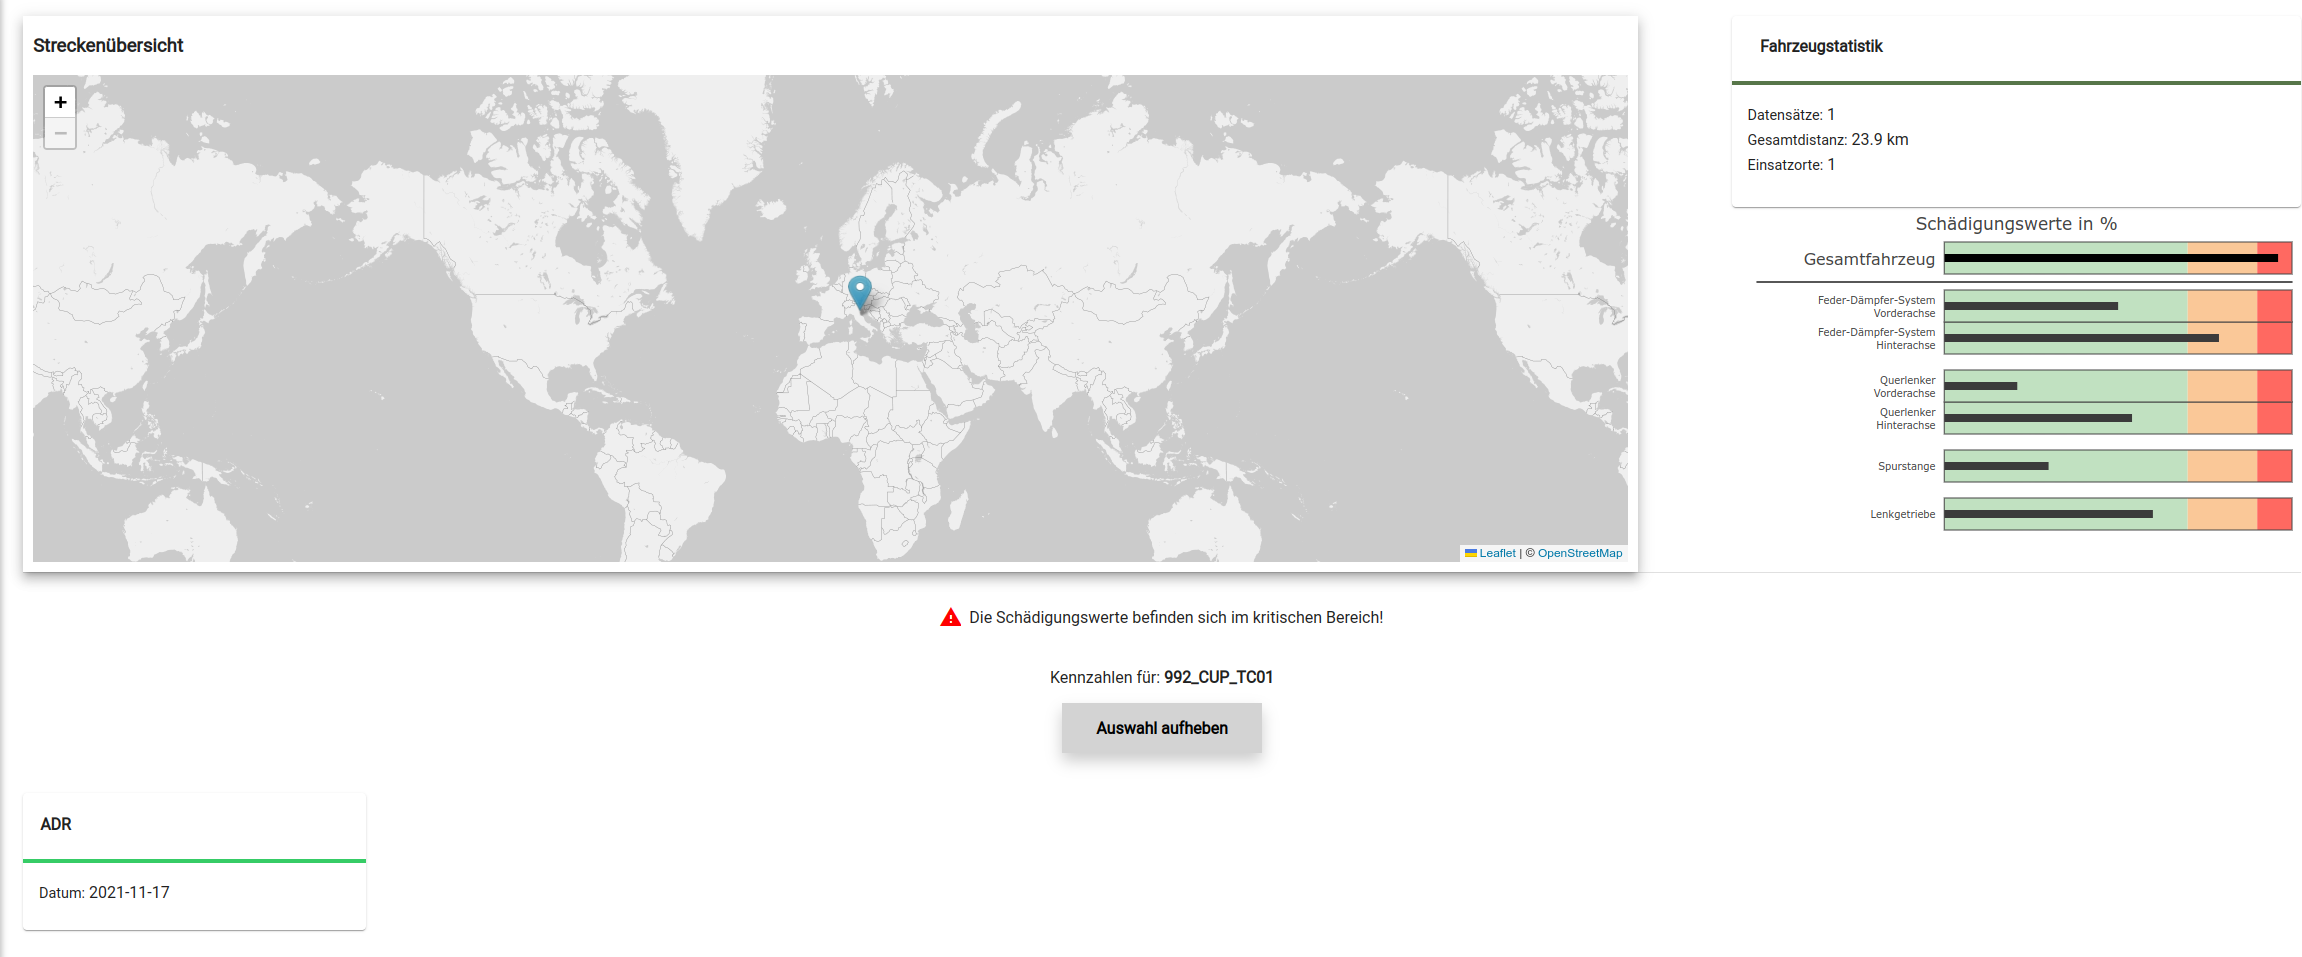
\includegraphics[width=0.8\textwidth]{gfx/Datenbasis_After.png}}
\caption{Datenbasis mit Bullet-Chart und Warnung}
\label{fig:datenbasis_after}
\end{figure}
\noindent
Nach Implementation des Graphen und der Warnung sieht die Datenbasis wie  in Abbildung \ref{fig:datenbasis_after} dargestellt aus.

\subsection{Fahrzeugvisualisierung mit Einfärbungen passend zur prozentualen Schädigung}
\label{sec:vehicle-images}
1. Kontext verstehen:\\
Um dem Benutzer zu ermöglichen, auch visuell zu erkennen, wo welche Schädigungen vorhanden sind, wird eine Fahrzeugvisualisierung eingebaut. Da es sich bei den zu überwachenden Fahrzeugen immer um das gleiche Modell handelt, ist die Implementation einfach gehalten. Es soll eine Möglichkeit gegeben werden, die einzelnen Konzeptzeichnungen der Fahrzeuge zu betrachten, wobei die Bauteile mit hoher Schädigung ähnlich wie in der Bullet-Chart in \ref{section:Prozentuale_Schädigung} eingefärbt werden sollen.\\\\
\begin{figure}[h!]
\centering
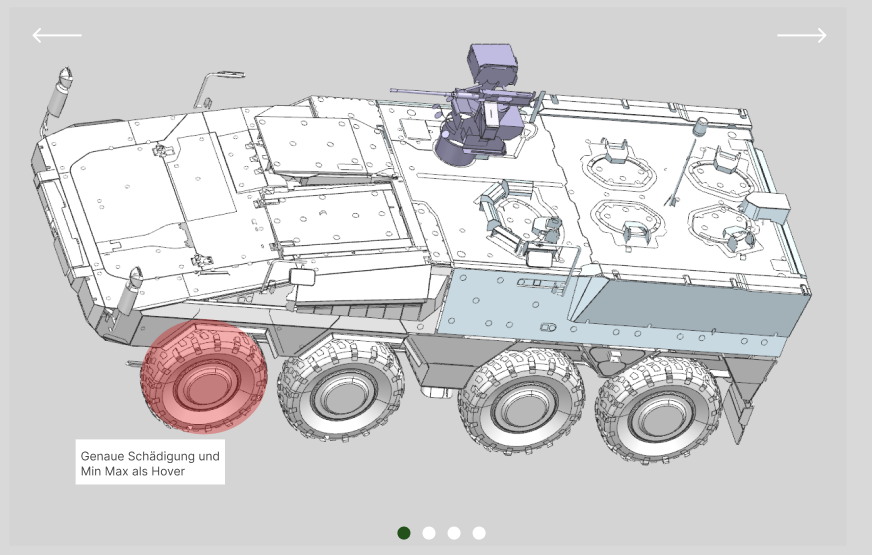
\includegraphics[width=0.8\textwidth]{gfx/vehicle_visualisation.png}
\caption{Prototyp der Fahrzeugvisualisierung}
\label{fig:vehicle_visualisation}
\end{figure}
\noindent
2. Darstellung wählen:\\
Als Darstellung eignet sich ein Karussell, in dem die Bilder angezeigt werden. Dann sollen die Bauteile eingefärbt werden und die Schädigung soll mit einem Hovereffekt mithilfe einer Image-Map ersichtlich werden. Bei dieser Darstellung handelt es sich zwar um keinen Graphen, Data-Storytelling kann aber trotzdem angewendet werden. Es wird in Figma \cite{FigmaGmbH.2024} ein Prototyp der Visualisierung erstellt (siehe Abbildung \ref{fig:vehicle_visualisation}).\\\\
3. Ordnung schaffen:\\
Um Ordnung zu schaffen, wird der Prototyp aus Figma \cite{FigmaGmbH.2024} dezenter implementiert. Dabei werden insbesondere als Pfeile zum Wechseln der Bilder solche gewählt, die weniger lang sind. Diese Pfeile werden in runde Buttons integriert. Bei der Darstellung, auf welchem Bild man sich im Karussell befindet, werden die Größe und die Farbe angepasst.\\\\
4. Aufmerksamkeit bündeln:\\
Die Aufmerksamkeit wird durch die farbigen Boxen auf der Image-Map gebündelt. Dabei wird anhand der Schädigung eine Farbe gewählt. Die Farben sind die gleichen wie in \ref{section:Prozentuale_Schädigung}, da auch in dieser Darstellung die Schädigung dargestellt wird. Es ist sinnvoll, die Farben über die gesamten Visualisierungen konstant zu halten, da der Benutzer in seinem Gehirn die Verbindung zwischen den Farben und dem Zustand der Schädigung herstellen wird. Mit dem Hovereffekt werden der Name der jeweiligen Komponente sowie die Schädigung angezeigt.\\\\
5. Geschichte erzählen:\\
Die Farben, die im Punkt 4. gewählt wurden, sowie die weiteren Graphen auf der Webseite dienen dazu, die Geschichte dieser Visualisierung zu erzählen. Analog ist der Call to Action bei \glqq roten\grqq{} Komponenten, diese zu warten oder zu erneuern. Die vollständige Visualisierung ist in Abbildung \ref{fig:vehicle_visualization_after} zu sehen. 
\begin{figure}[h!]
\centering
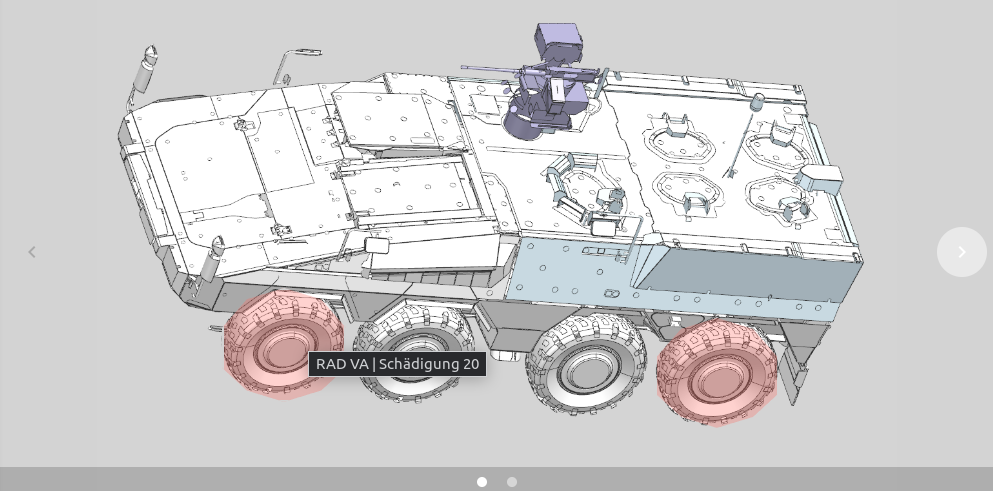
\includegraphics[width=0.8\textwidth]{gfx/vehicle_visualisation_after.png}
\caption{Fahrzeugvisualisierung der Baugruppen mit Hovereffekt}
\label{fig:vehicle_visualization_after}
\end{figure}
\noindent
Die Visualisierung ist in zwei verschiedene Arten von Bildern eingeteilt: zum einen die Bilder, die die Baugruppen des Fahrzeugs zeigen, und zum anderen die Bilder, die die einzelnen Komponenten in den jeweiligen Baugruppen darstellen. Es wird bei dieser Visualisierung also eine Art Drill-down genutzt, um die verschiedenen Komponenten darzustellen. Zunächst sind nur die Bilder der Baugruppen im Karussell zu sehen. Wird aber auf eine Baugruppe geklickt, wird ein weiteres Bild zum Karussell hinzugefügt und das Karussell zu der passenden Position navigiert. Dadurch lässt sich die Auswirkung der einzelnen Komponenten auf die Baugruppen wirkungsvoll darstellen. Da sich die Bilder bei Hinterachse und Vorderachse kaum unterscheiden, wurde zum einfacheren Verständnis ein Titel hinzugefügt. Die Komponentenbilder sind in Abbildung \ref{fig:vehicle_visualization_detail} dargestellt.
\begin{figure}[h!]
\centering
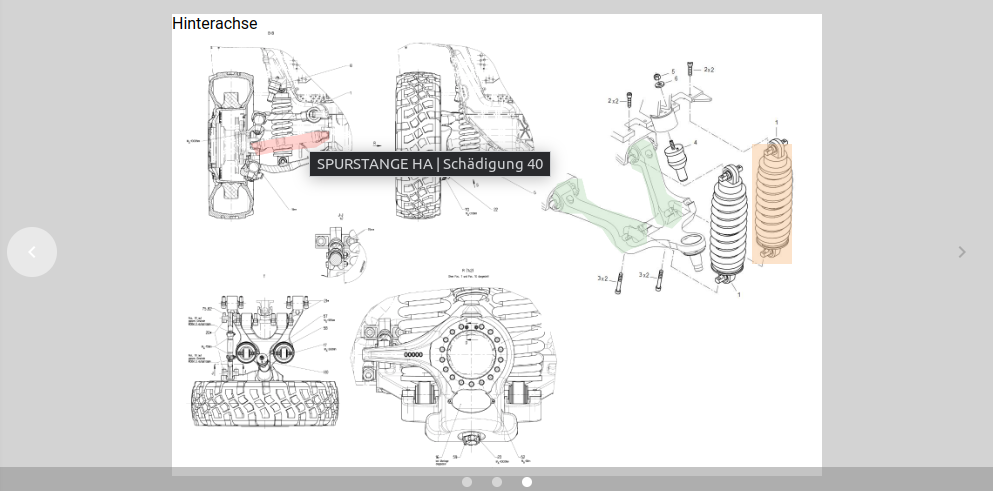
\includegraphics[width=.8\textwidth]{gfx/vehicle_visualisation_detail.png}
\caption{Fahrzeugvisualisierung der Komponenten mit Hovereffekt}
\label{fig:vehicle_visualization_detail}
\end{figure}
\subsection{Fingerprints}
1. Kontext verstehen:\\
Bei den von monalysis entwickelten Fingerprints \cite{MichaelStadele.2008} handelt es sich um eine Darstellung, die aus jeweils drei Teilen besteht. Dabei wird beschrieben, wie sich die Fahrbahn zum Bauteil verhält beziehungsweise wie belastend die Straßen sind. Außerdem können mit den Fingerprints Fahrmanöver erkannt werden \cite{MichaelStadele.2008}. Die drei Teile setzen sich zusammen aus aX, aY und aZ, die die verschiedenen Raumrichtungen beschreiben. Jede dieser Raumrichtungen hat wiederum Frequenzbänder, die dargestellt werden sollen. Insgesamt gibt es pro Raumrichtung neun Frequenzbänder in diesem Anwendungsfall. Die Frequenzbänder werden als aX1--aX9 bezeichnet, wobei gilt: Je niedriger die Zahl, desto niederfrequenter ist die Messung. Zusätzlich soll noch die gesamte Schädigung pro Raumrichtung dargestellt werden. Die Fingerprints wurden deswegen entwickelt, weil man alleine über die Schädigung keinen Überblick über die niederfrequenten Bereiche der Messung hat. Durch die Darstellung der Fingerprints wird die Intensität der Straße erkennbar.\\\\
2. Darstellung wählen:\\
Als Darstellung für die Fingerprints eignet sich eine Linechart. Die drei Raumrichtungen werden zwar separat betrachtet, aber es ist doch wichtig, die Verläufe vergleichen zu können. Für die Fingerprints ist bereits eine Implementation vorhanden, auf welcher der Graph basiert (\ref{fig:fingerprints_first}).
\begin{figure}[!h]
    \centering
    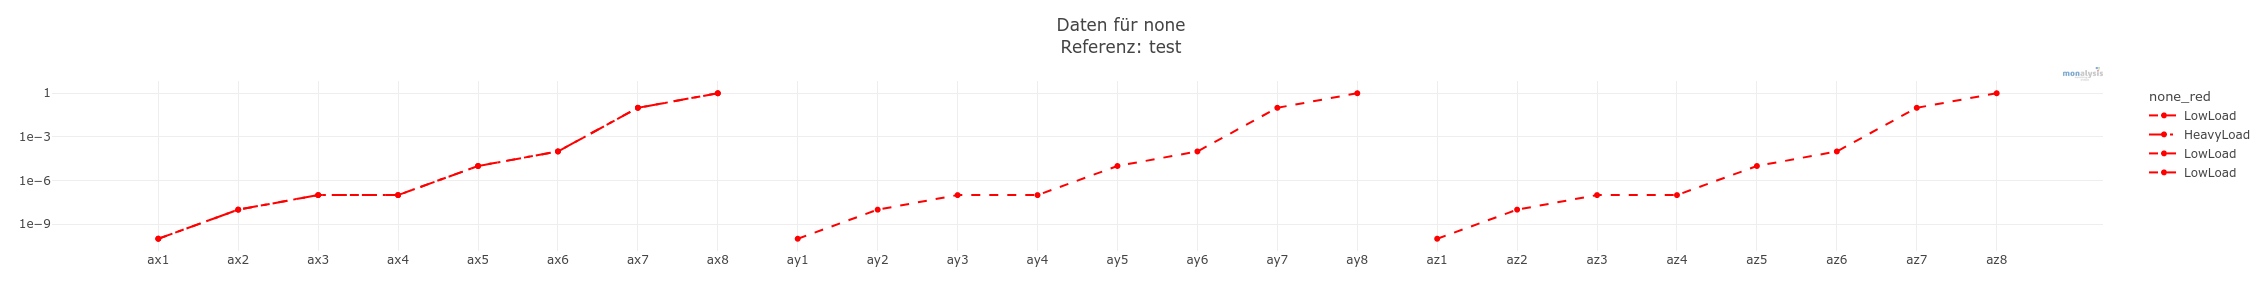
\includegraphics[width=1\linewidth]{gfx/fingerprints_first.png}
    \caption{Bereits vorhandene Implementation der Darstellung der Fingerprints}
    \label{fig:fingerprints_first}
\end{figure}
\\\\3. Ordnung schaffen:\\
Im Sinne des Data-Storytelling-Punkts „Ordnung schaffen“ ist die bereits vorhandene Implementierung gut gelungen. Bei den Gridlinien werden die vertikalen Linien für aX, aY und aZ entfernt. Ebenso wird der Titel des Graphen überarbeitet. Für diese Implementation ist weder eine Region noch eine Referenz vorgesehen, also kann der Titel entfernt werden. Die Implementation der Linien wird überarbeitet, sodass die Linien als einfache Linien dargestellt werden können, anstatt in verschiedene Richtungen unterbrochen. Das beruhigt den Graphen im Allgemeinen. Die Implementation wird weiterhin angepasst, sodass keine mehrfachen Einträge in der Legende sichtbar sind. Die Position des Logos ist in diesem Graphen gut gelungen, da weder die Daten noch das Logo überdeckt werden. Der Graph wird als zwei verschiedene Varianten implementiert: Es ist möglich, mehrere Fingerprints in einem Graphen darzustellen oder diese mit einem Toggle voneinander zu trennen und separate Graphen zu rendern. Zudem wird die Limitation festgelegt, dass nur fünf Fingerprints gleichzeitig dargestellt werden können.\\\\
4. Aufmerksamkeit bündeln:\\
Um die Aufmerksamkeit des Benutzers auf die einzelnen Raumrichtungen zu lenken, werden Annotations erstellt, die den im Punkt „Ordnung schaffen“ entfernten Titel ersetzen. In der Legende wird der erzeugte Name des Fingerprints dargestellt, der sich aus Fahrzeugname, Erprobungsbahn, gefahrener Geschwindigkeit und Laufleistung zusammensetzt. Dadurch sieht man auf einen Blick, welche Parameter für die Linie wichtig sind. Ansonsten sollen die Linien farbig gekennzeichnet werden. Da es sich um bis zu fünf Linien handeln kann und diese nur durch ihre Farben zu unterscheiden sind, werden die klassischen Farben Rot, Grün, Blau, Schwarz und Grau gewählt. Wird ein einzelner Fingerprint dargestellt, soll dieser im gleichen Grau gefärbt werden wie die Zeitreihen \ref{sec:timeseries}.\\\\
5. Geschichte erzählen:\\
Die Fingerprints sind ein Analysewerkzeug, bei dem es relevant ist, wie nah die gemessenen Daten an der Zahl Eins sind, also wie nah die ausgewählte Messstelle sich an 100\,\% Erprobung befindet. Dazu wird das Grid bei der Zahl Eins hervorgehoben. Dadurch kann der Benutzer direkt erkennen, wie nah sich die Messstelle der Erprobung nähert, und somit auch abschätzen, wann diese Messstelle potenziell ausgetauscht oder gewartet werden soll. Mit diesen Anpassungen wird die Fingerprintdarstellung in \ref{fig:fingerprints_finished} abgebildet.
\begin{figure}[!h]
    \centering
    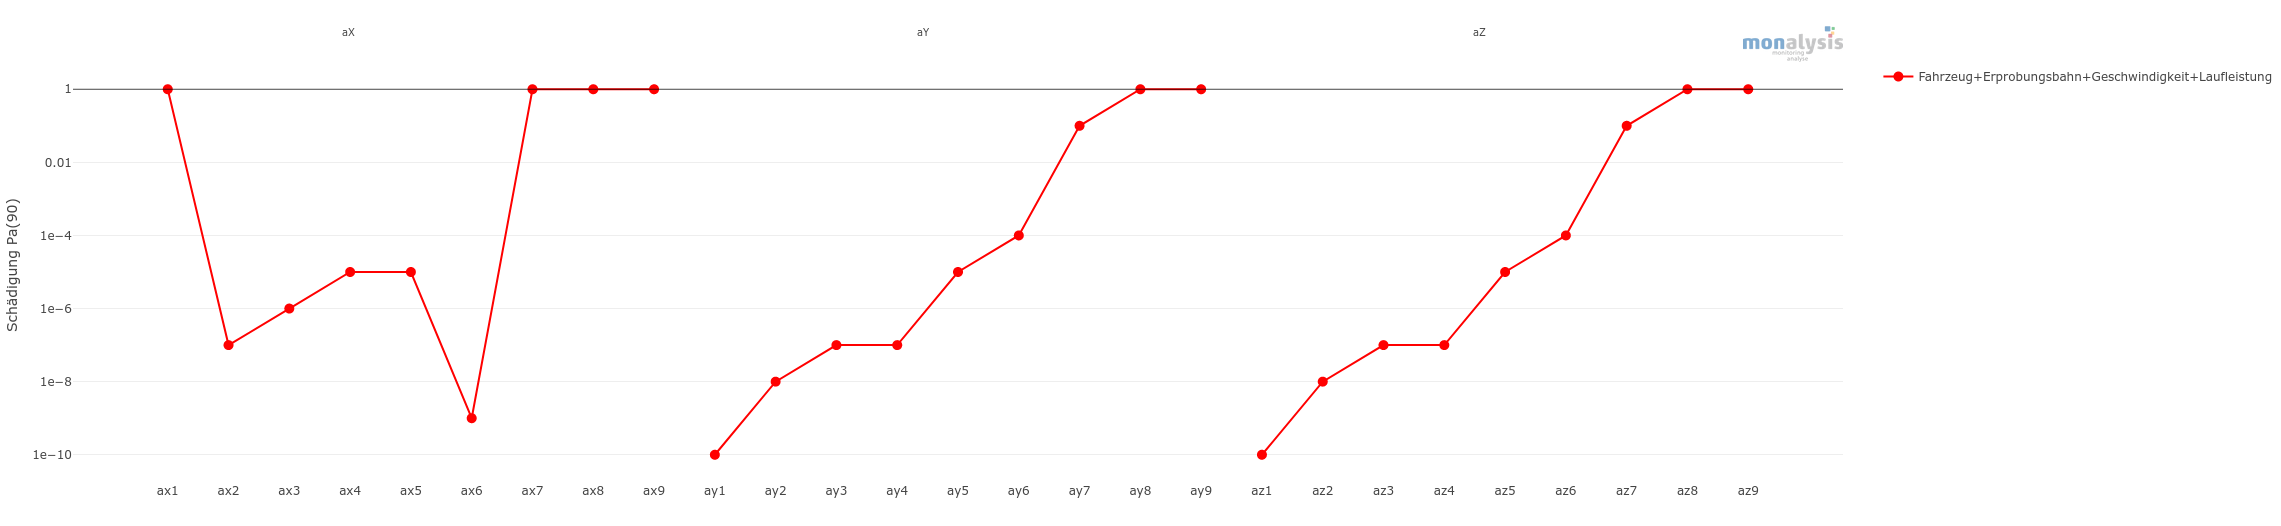
\includegraphics[width=1\linewidth]{gfx/fingerprints_finished.png}
    \caption{Vollständige Darstellung der Fingerprints}
    \label{fig:fingerprints_finished}
\end{figure}
\subsection{Dauerlauferprobung}
\label{section:dauerlauferprobung}
1. Kontext verstehen:\\
Die Dauerlauferprobung soll ein Graph sein, der die Schädigung über die Zeit (oder die bereits gefahrenen Kilometer) der Erprobung darstellt, zudem die Grenze, ab der die betrachtete Messstelle oder das Gesamtfahrzeug nicht mehr erprobt ist. Die Dauerlauferprobung ist also eine Ansammlung von Werten über einen Zeitraum und dazu eine spezifische Grenze. Es gibt für die Dauerlauferprobung zwei verschiedene Anzeigen: eine, die in einem Graphen die gesamte kumulierte Schädigung anzeigt, und eine, die sich auf die unterschiedlichen Raumrichtungen aX, aY und aZ beschränkt. Im Folgenden wird der Graph für die gesamte kumulierte Schädigung betrachtet. Es soll möglich sein, bei der x-Achse umzustellen, ob die Zeit betrachtet wird oder die gefahrenen Kilometer. Insgesamt sind in einer Dauerlauferprobung bei diesem Anwendungsfall immer 16\,000\,km zu fahren.\\\\
2. Darstellung wählen:\\
Es bietet sich an, den Graphen als einen Linegraphen zu implementieren, da es sich um eine Ansammlung von Werten über die Zeit handelt. Dadurch lässt sich auch die Grenze der Erprobung gut hervorheben.\\\\
 3. Ordnung schaffen:\\
Es wird bei der Erstellung des Graphen von dem plotly.js-Beispiel für einen Linegraphen ausgegangen \cite{Plotly.2024}. Da bei dieser Darstellung das Interesse bei dem Verlauf sowie dem aktuellen Stand der Dauerlauferprobung liegt, bietet es sich an, die Range des Graphen zu erhöhen, damit der aktuelle Zeitpunkt zentrierter im Graph ist und mehr hervorgehoben wird. Zusätzlich wird ein Titel hinzugefügt, damit der Benutzer direkt weiß, was dieser Graph darstellt. Da der Wert der Messung im Vordergrund steht, wird, um den Visual Clutter zu entfernen, das Grid für die x-Werte entfernt. Der Graph vor und nach dem Ordnungschaffen ist in Abbildung \ref{fig:dauerlauferprobung_before} dargestellt.
\begin{figure}[!h]
    \centering
    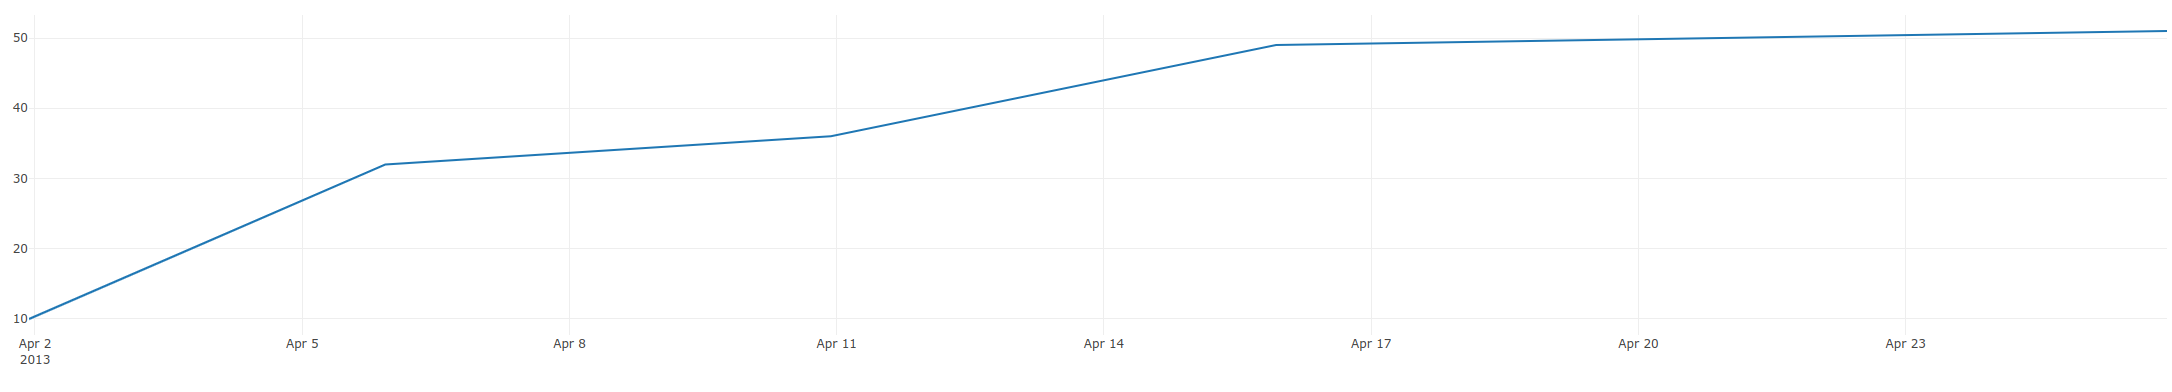
\includegraphics[width=\linewidth]{gfx/dauerlauferprobung_before.png}
        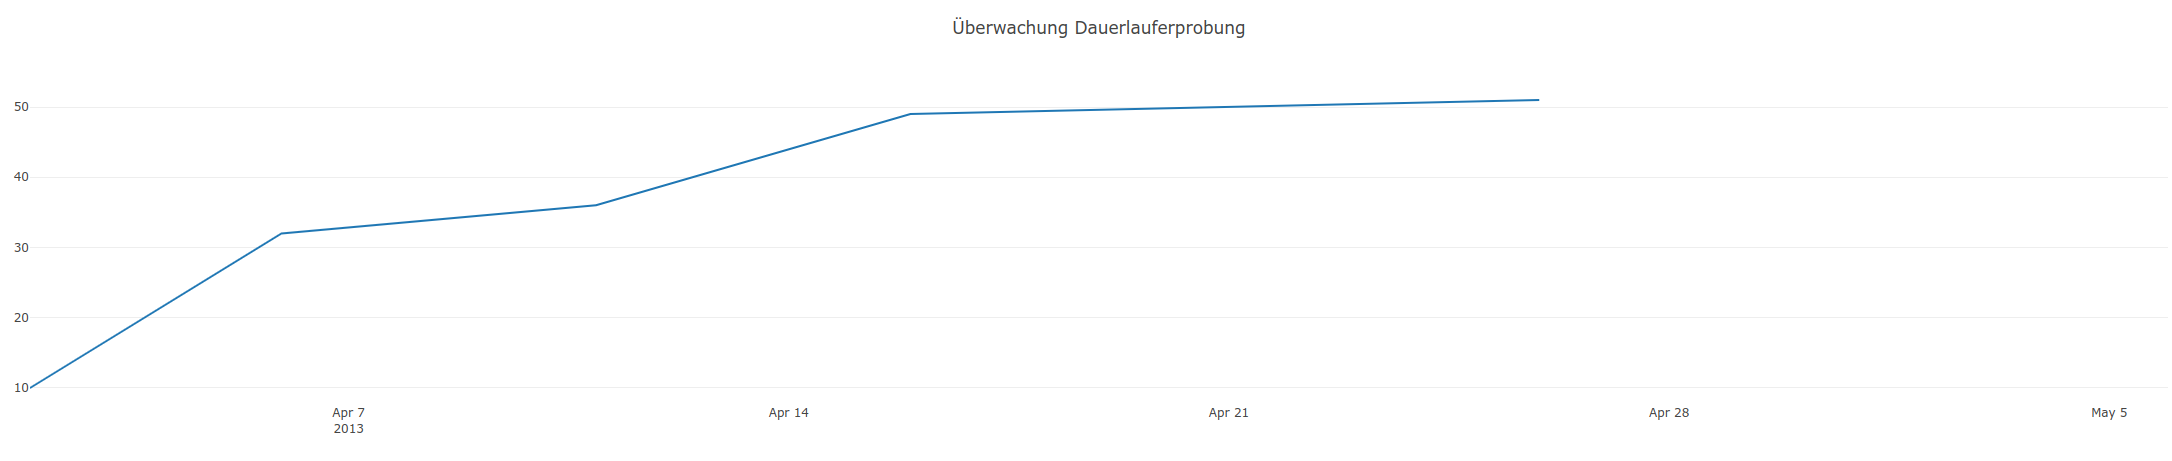
\includegraphics[width=1\linewidth]{gfx/dauerlauferprobung-after.png}
    \caption{Dauerlauferprobung vor und nach dem Ordnungschaffen}
    \label{fig:dauerlauferprobung_before}
\end{figure}
\\\\
 4. Aufmerksamkeit bündeln:\\
Sinnvoll ist es, den Wert der Grenze in dem Graphen darzustellen. Dadurch wird die Aufmerksamkeit des Benutzers nicht nur gebündelt, sondern der Benutzer kann direkt erkennen, wie weit das Bauteil schon erprobt ist. Durch den bereits vorhandenen Verlauf des tatsächlichen Schadens kann der Benutzer auch ungefähr abschätzen, wann die Grenze überschritten werden könnte. Die Messungen können zwar in unregelmäßigen Abständen durchgeführt werden, aber es kann davon ausgegangen werden, dass sich die Schädigung pro Prüfung ungefähr gleich verhält. Die Linie des Graphen wird zusätzlich passend zu den weiteren Graphen auf der Webseite eingefärbt. Das Ergebnis ist in Abbildung \ref{fig:dauerlauferprobung_aufmerksamkeit} abgebildet.
\begin{figure}[!h]
    \centering
    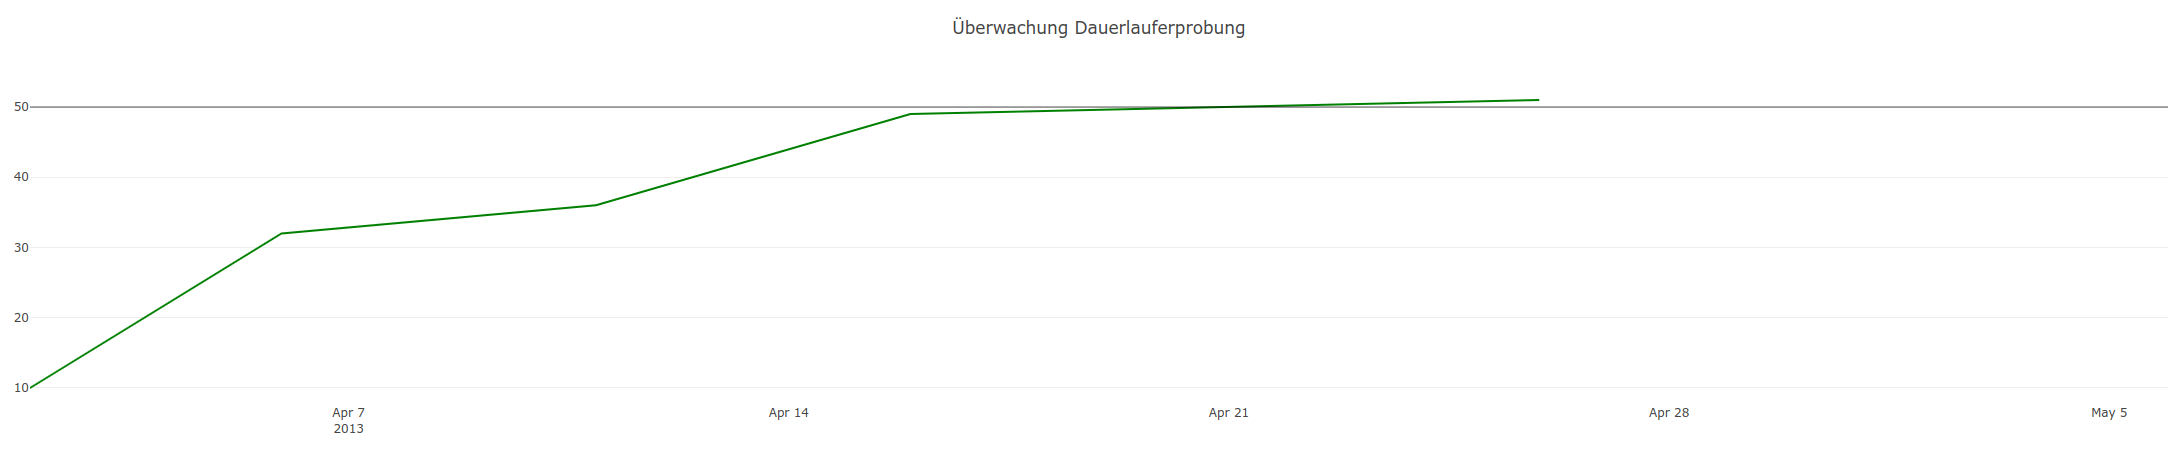
\includegraphics[width=1\linewidth]{gfx/dauerlauferprobung_aufmerksamkeit.png}
    \caption{Dauerlauferprobung mit eingezeichneter Grenze und passender Farbe}
    \label{fig:dauerlauferprobung_aufmerksamkeit}
\end{figure}
\\\\
 5. Geschichte erzählen:\\
Wichtig ist bei der Dauerlauferprobung zum einen, wann der tatsächliche Schaden die erprobte Grenze überschreitet. Zum anderen ist interessant, wann eine hohe Steigung in dem Verlauf der Erprobung erreicht wird. Wenn die erprobte Grenze überschritten wird, wird der Schnittpunkt der erprobten Linie und der Schäden gesucht. Deswegen ist es sinnvoll, diesen durch die Unterlegung von Farbe hervorzuheben. In plotly.js gibt es keine eingebaute Funktion, um den Schnittpunkt von zwei Linien herauszufinden. Aber da sich die Linie der Erprobung konstant auf einer Höhe befindet, kann man prüfen, wann diese Höhe überschritten wird, und den Punkt nach der Überschreitung und den Punkt vor der Überschreitung als Grenzen für die Einfärbung nutzen. Die Darstellung, wenn die Grenze überschritten wird, ist in Abbildung \ref{fig:dauerlauferprobung_story} zu sehen. Für das Erreichen einer gewissen Steigung kann die Trenderkennung genutzt werden. Die Werte der Dauerlauferprobung werden immer ansteigen, weil ein Fahrzeug keine negativen Kilometer zurücklegen kann. Also eignet sich die Funktion zum Erkennen der Aufstiege \texttt{detectRisesInData} aus \ref{subsection:risesAndFalls}, wobei eine Distanz von 0 zwischen dem Start- und Endpunkt angegeben wird. Auch der gleitende Durchschnitt ist für diesen Anwendungsfall nicht unbedingt nötig, da keine kleinen Abstiege ausgeglichen werden müssen. Als Eingabe für den gleitenden Durchschnitt bei der Funktion können auch einfach die richtigen Werte aus der Dauerlauferprobung weitergegeben werden.\\\\
\begin{figure}[!h]
    \centering
    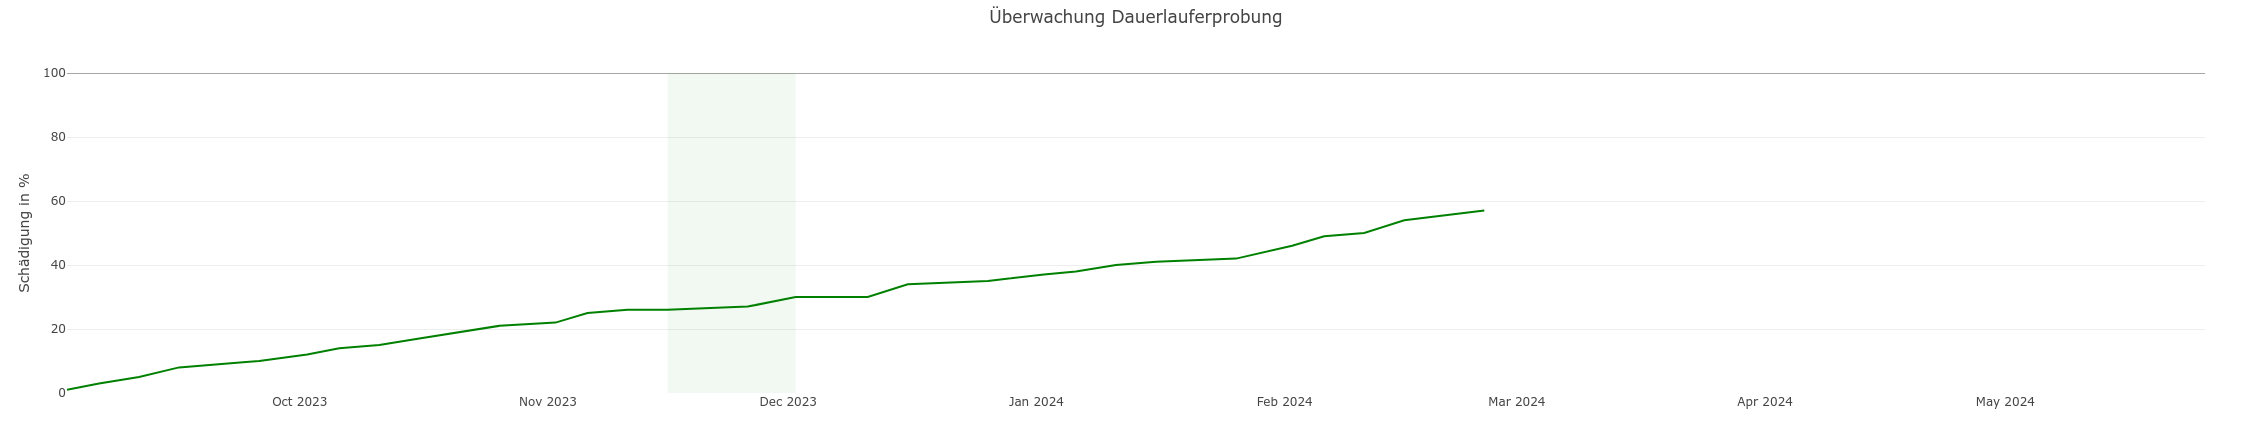
\includegraphics[width=1\linewidth]{gfx/dauerlauferprobung_story.png}
    \caption{Dauerlauferprobung mit den erkannten Aufstiegen}
    \label{fig:dauerlauferprobung_story}
\end{figure}

\subsection{Kumulierte Schädigung von allen gemessenen Durchfahrten}
\label{section:schaedigung}
1. Kontext verstehen:\\
Dieser Graph soll als Einstiegspunkt für die Analysen gelten. Es soll eine Übersicht über die verschiedenen gefahrenen Runden in den Daten geben. Dabei sollen pro gemessener Fahrt jeweils die Minimal-, Maximal- und Schädigungswerte der Messstellen dargestellt werden. Der Graph soll eine Bar-Chart sein, damit die verschiedenen Größen untereinander verglichen werden können. Die Balken sollen horizontal angeordnet sein. Ein Fahrzeug kann bis zu 50 Messstellen haben. Die Daten für diesen Graphen werden als Typ \texttt{ProfileData} aus \ref{appendix:graph_types} formatiert. 
\\\\
2. Darstellung wählen:\\
Ein Requirement für den Graphen ist, dass die Darstellung in einem Balkendiagramm erfolgen soll. Das Diagramm soll die Balken von links nach rechts anordnen. Dadurch kann bei der Betrachtung direkt verglichen werden, wie die einzelnen Messstellen zueinander stehen. Hierbei können sogleich zu hohe Werte erkannt werden.\\\\
3. Ordnung schaffen:\\
Dieser Graph basiert auf einer bereits vorhandenen Implementation der Darstellung. Diese Implementation ist in Abbildung \ref{fig:schaedigung_before} zu sehen.
\begin{figure}[!h]
    \centering
    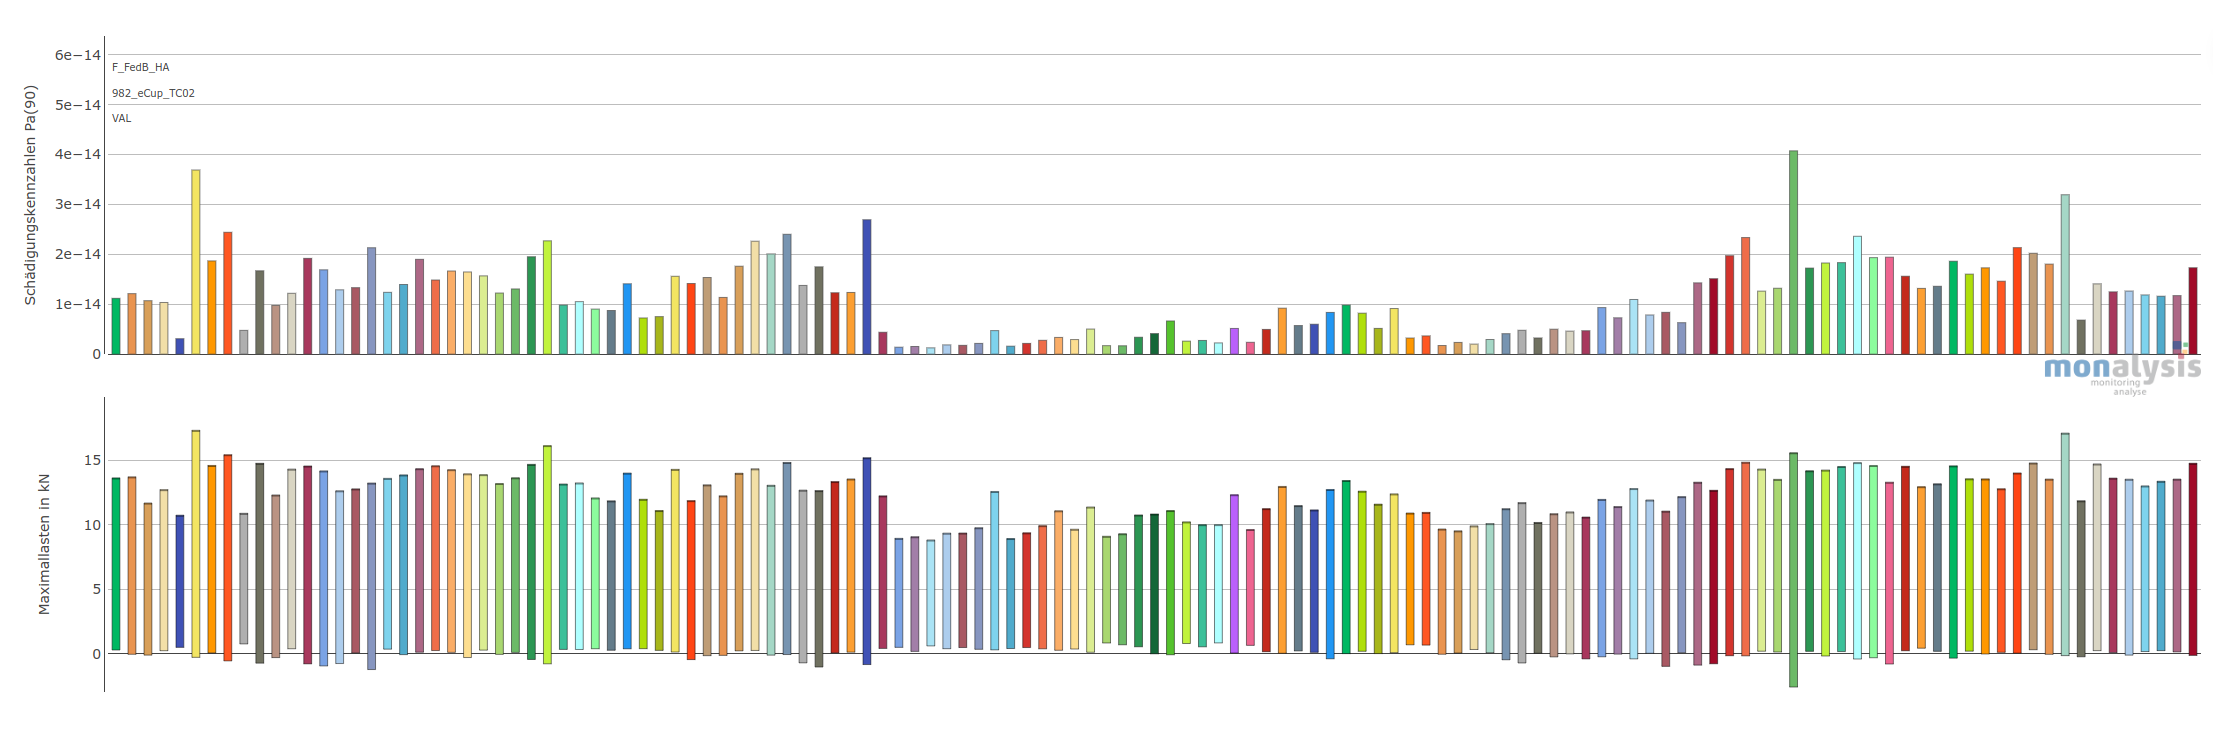
\includegraphics[width=1\linewidth]{gfx/schaedigung.png}
    \caption{Darstellung vor dem Data-Storytelling}
    \label{fig:schaedigung_before}
\end{figure}
Dadurch, dass in dem Graphen potenziell viele Messstellen dargestellt werden müssen, ist es umso wichtiger, die bisherige Darstellung zu vereinfachen. Zunächst werden die Farben aus den Balken entfernt, da laut \cite{BO.2019} Farben, je nachdem wie hell oder dunkel, ob es sich beispielsweise also um Grün oder Gelb handelt, unterschiedliche Effekte auf das Gehirn haben. So unterscheiden sich beispielsweise Grün oder Blau von den wärmeren Farben wie Rot oder Orange \cite{BO.2019}, da diese eher die Aufmerksamkeit des Benutzers auf sich ziehen. Da die Farben aber ursprünglich zufällig zugeordnet werden, kann nicht kontrolliert werden, welchen Balken warme und welchen kühle Farben zugewiesen werden. Deswegen werden in dieser Implementation die Balkenfarben entweder in einem einfachen Grau gehalten oder es können mithilfe eines zufälligen Grautongenerators verschiedene Grautöne generiert werden. In der Implementation ist ein Generator vorhanden, der auf \cite{Moob.2017} basiert, aber durch die Menge der darzustellenden Werte ist zunächst die Variante mit einem gleichen Farbton implementiert worden. Die Achsen haben bereits ein vereinfachtes Design; wenn zusätzlich die horizontalen Gridlinien entfernt werden, fällt das Vergleichen der Höhe der Balken schwerer. Das Logo der Firma sollte neu platziert werden, damit keine Balken überschnitten werden können. Auch die Platzierung der Achsentexte, \glqq Schädigungskennzahlen Pa(90)\grqq{} und \glqq Maximallasten in kN\grqq{}, werden durch die automatische Platzierung von plotly.js nicht genau untereinander gesetzt. Deswegen werden die Achsentexte durch Annotations ersetzt, die den gleichen Text darstellen, aber nicht abhängig von den Werten in der Achse platziert werden.\\\\
4. Aufmerksamkeit bündeln:\\
Aus den Experteninterviews konnte kombiniert werden, dass bei diesem Graphen hauptsächlich ein grober Überblick über die Daten und deren Beschaffenheit geschaffen werden soll. Zudem achten die Experten auf besonders hohe Balken, sowohl bei der Schädigung als auch bei den Minimal- und Maximalwerten. Es gibt dafür den internen Begriff „Topfilter“. Bisher wurde dieser Topfilter wie eine Auswahl gestaltet, bei der der Benutzer auswählen kann, wie viele Top-Werte dargestellt werden sollen. Dabei gibt es die Auswahlmöglichkeiten 1, 3, 5 und 10. Diese Top-Werte beziehen sich auf die Schädigungswerte. Sollten der  minimale und maximale Wert nicht unter den Top-Werten sein, werden diese zusätzlich hinzugefügt. Es werden also maximal 12 Werte als Top-Werte klassifiziert. Um die Aufmerksamkeit des Benutzers direkt auf die Top-Werte zu lenken, die laut den Experten der interessanteste Aspekt in der Darstellung sind, sollten die ersten Top-Werte gekennzeichnet werden, ohne dass der Benutzer eine Auswahl treffen müsste. Es bietet sich an, die Top-Werte einzufärben, da der Graph nun keine Farben mehr darstellt. Durch die Farbe fällt auf, welcher Wert für die Analyse interessant ist. Die Top-Werte lassen sich je nach Schädigung sortieren, und anhand dieser Sortierung wird der Farbton gewählt. Je heller die Farbe, desto höher die Schädigung, was in Kombination mit den grauen Balken der nicht als Top-Werte klassifizierten Werte zu einem Herausstechen der Top-Werte führt.
\begin{figure}[!h]
    \centering
    \includegraphics[width=1\linewidth]{gfx/schädigung_agter.png}
    \caption{Schädigungsdarstellung nach dem Ordnungschaffen und Aufmerksamkeitbündeln}
    \label{fig:schaedigung_after}
\end{figure}
\noindent
Dieser Effekt ist deutlich in Abbildung \ref{fig:schaedigung_after} zu betrachten. Es soll trotzdem noch die Möglichkeit gegeben sein, die Balken im Graphen auf die Top-Werte zu reduzieren. Durch diese Reduzierung kann der Benutzer die einzelnen interessanten Kanäle betrachten. Diese Reduzierung vom gleichen Datensatz ist in Abbildung \ref{fig:schädigung_reduziert} dargestellt. Da bei der Reduzierung nur maximal 12 Werte dargestellt werden, ist es möglich, bei der Darstellung einige Informationen hinzuzufügen. Die genauen Schädigungswerte werden auf den Balken eingeblendet, damit zu erkennen ist, welche Schädigungszahlen betrachtet werden. In plotly.js lässt sich für diesen Text nur eine Farbe angeben. Wenn die Balken aber beispielsweise dunkelgrün sind, ist schwarze Schrift nur schwer zu erkennen. Dafür wurde mithilfe von \cite{Alnitak.2012} eine Funktion entwickelt, die den Schädigungstext je nach Farbe des Balkens einfärbt. Wenn es weißer Text wird, wird bei diesem ein schwarzer Rand hinzugefügt.
\begin{figure}[!h]
    \centering
    \includegraphics[width=1\linewidth]{gfx/schädigung_reduziert.png}
    \caption{Reduzierung des gleichen Datensatzes wie in Abbildung \ref{fig:schaedigung_after}}
    \label{fig:schädigung_reduziert}
\end{figure}
\\\\5. Geschichte erzählen:\\
Der Graph erzählt die Geschichte, wie die verschiedenen Messungen auf den Messstellen ausgewertet wurden. Dabei ist das Erzählen einer Geschichte  schwierig, weil keine Messung als schlecht oder gut gelten kann, nur als interessant. Durch die farbliche Hervorhebung des Top-Wertes wird in gewisser Weise die Geschichte erzählt, da dieser Wert der interessanteste ist. Auch ein Call to Action ist so weit definierbar, dass die farbliche Hervorhebung dazu einlädt, die weiteren Funktionen zu nutzen. Damit kann analysiert werden, weshalb bei dieser Messung der höchste Wert aufgetreten ist. Dafür können über den Graphen durch einen Klick auf den Balken sowohl die Kollektive als auch die Zeitreihen angefordert werden. Die Kollektive eignen sich durch ihre unveränderliche Darstellung in der Betriebsfestigkeit \cite{Gotz.2020} und ihre Natur in der einfachen Darstellung von Ausschlägen in einem Messsignal \cite{PatrickPfeiffer.17.10.2022}  wenig zum Data-Storytelling, da es keinen Call to Action und auch keine Geschichte gibt, außer den Verlauf des Graphen. Die Zeitreihen hingegen eignen sich durch die Trenderkennung hervorragend für das Data-Storytelling.
% \subsection{Kollektive}
% 1. Kontext verstehen:\\
% Kollektive sind eine feste Größe in der Betriebsfestigkeit \cite{Gotz.2020}. Bei den Kollektiven werden laut \cite{PatrickPfeiffer.17.10.2022} lediglich die höchsten Ausschläge des Messsignals betrachtet. Dabei werden verschiedene Zählmethoden verwendet. In diesem Use Case gibt es die folgenden Darstellungen:
% \begin{description}
%   \item[Level Crossing (deut. Klassengrenzenüberschreitungszählung)] \hfill \\ 
%   Das Level Crossing Verfahren \glqq beschreibt die Häufigkeit, mit welcher die Last-Zeit-Funktion [(Zeitreihe oder Messung)] zuvor definierte Klassen überschreitet. [Deswegen] kann ein schneller Überblick über gemessene Minima und Maxima gewonnen werden\grqq{} \cite{PatrickPfeiffer.17.10.2022} \cite{TaylanKaplan.01.04.2015}.
%   \item[Range Pair (deut. Bereichspaarzählung)] \hfill \\ 
%   Bei der Range Pair Zählung werden \glqq von Minima aufwärts und von Maxima abwärts Spannen erfasst\grqq{} \cite{BenediktMundl.25.08.2010}. Bei dieser Darstellung werden die Amplituden und Häufigkeiten erfasst und dargestellt \cite{TaylanKaplan.01.04.2015}. 
%   \item[Time at Level (deut. Verweildauerzählung)] \hfill \\ 
%   Laut \cite{PatrickPfeiffer.17.10.2022} wird die Time at Level Zählung \glqq vorwiegend für die Analyse von Fahr- oder Maschinenzuständen angwandt\grqq{}. Dabei wird die Dauer, in der sich das Lastgeschehen in den jeweiligen Klassen aufhält gezählt \cite{PatrickPfeiffer.17.10.2022}.
% \end{description}
% \noindent
% 2. Darstellung wählen:\\
% Als Darstellung wird wie in der Betriebsfestigkeit \cite{Gotz.2020} üblich ein Linegraph genutzt. Die standardmäßige Darstellung der verschiedenen Zählmethoden ist in  \ref{fig:countingMethods} zu sehen. 
% Da es sich bei der Zielgruppe des Graphen ausschließlich um Ingenieure handelt, die sich mit dem Thema der Betriebsfestigkeit auskennen, wäre es für das Ziel des Data Storytellings, die Daten schnell an den Benutzer zu transportieren hinderlich, sich nicht auf diese bewährte Darstellungsart festzulegen.
% \begin{figure}[h!]
% \centering
% 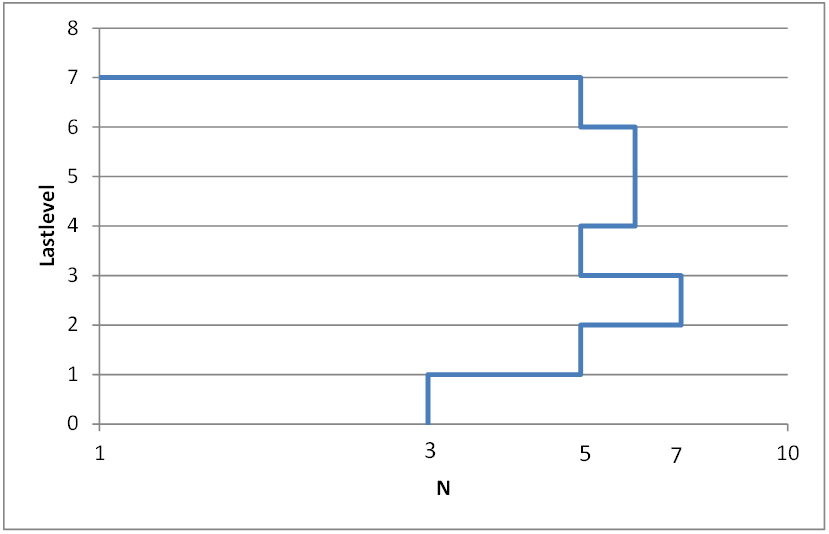
\includegraphics[width=0.3\textwidth]{gfx/level-crossing.png} 
% 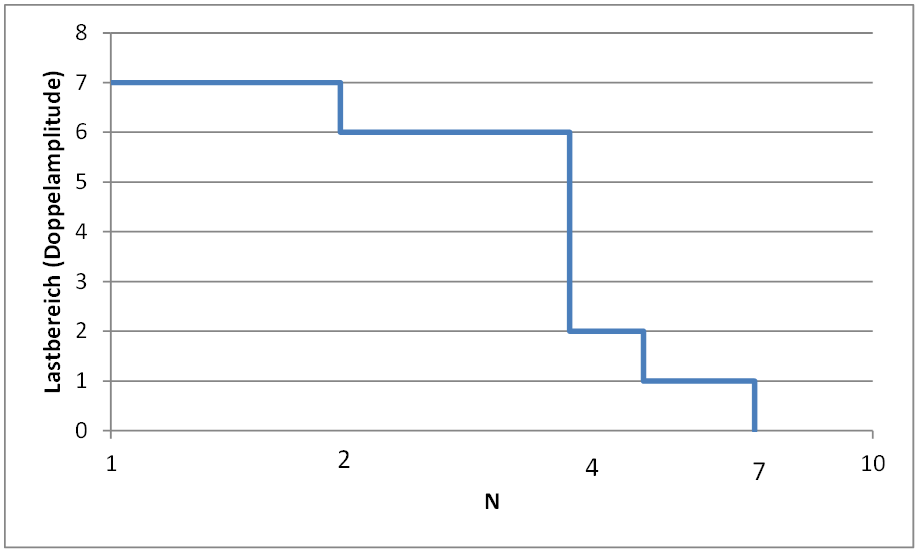
\includegraphics[width=0.3\textwidth]{gfx/range-pair.png}
% 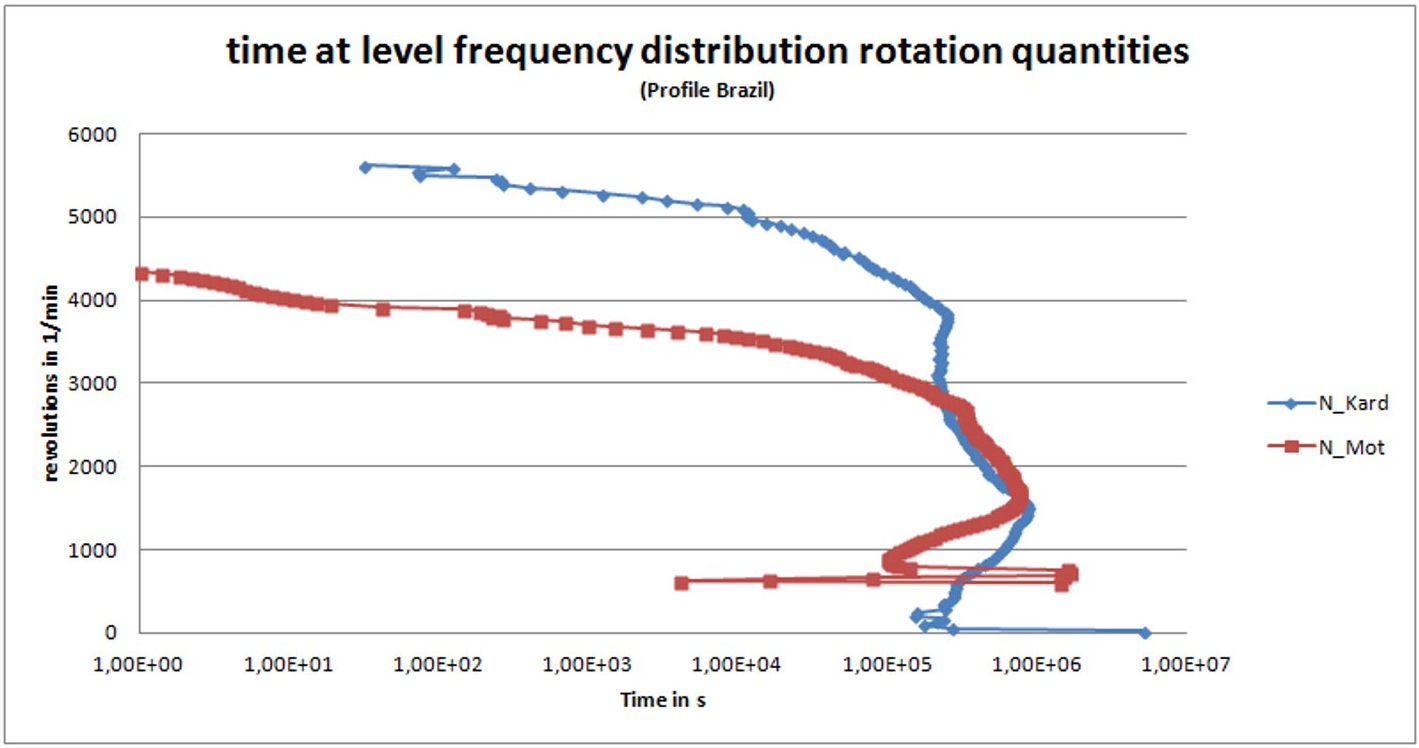
\includegraphics[width=0.3\textwidth]{gfx/time-at-level.png}
% \caption{Level Crossing, Range Pair und Time at Level vor Einsatz des Data Storytellings \cite{BenediktMundl.2023}}
% \label{fig:countingMethods}
% \end{figure}
% \noindent
% 3. Ordnung schaffen:\\
% 4. Aufmerksamkeit bündeln:\\
% 5. Geschichte erzählen:\\
\subsection{Zeitreihen}
\label{sec:timeseries}
1. Kontext verstehen: \\
Die Zeitreihen werden dazu genutzt, die Kräfte, die auf die Bauteile wirken, detailreich darzustellen. Die Kräfte werden meistens in einer Frequenz von 500\,Hz über einen festen Zeitraum gemessen. Eine Zeitreihe ist ein Werkzeug aus der Statistik, das allgemein dazu verwendet wird, Werte über den Verlauf eines Zeitraums darzustellen \cite{Billeter.1981}.
\\\\
2. Darstellung wählen:\\
Laut \cite{Gotz.2020} sind Zeitreihen ein fester Bestandteil des Bereiches der Betriebsfestigkeit. Deswegen ergibt es Sinn, nicht von der allgemeinen Darstellung abzuweichen. Zeitreihen werden ausschließlich als Linegraph dargestellt, da es sich klar um einen einzelnen Wert über eine bestimmte Zeit handelt. Es ist auf keinen Fall sinnvoll, von den bereits etablierten Graphen abzuweichen, da das den Cognitive Load für den Benutzer erhöhen würde.
\\\\
3. Ordnung schaffen:\\
\begin{figure}[h!]
\centering
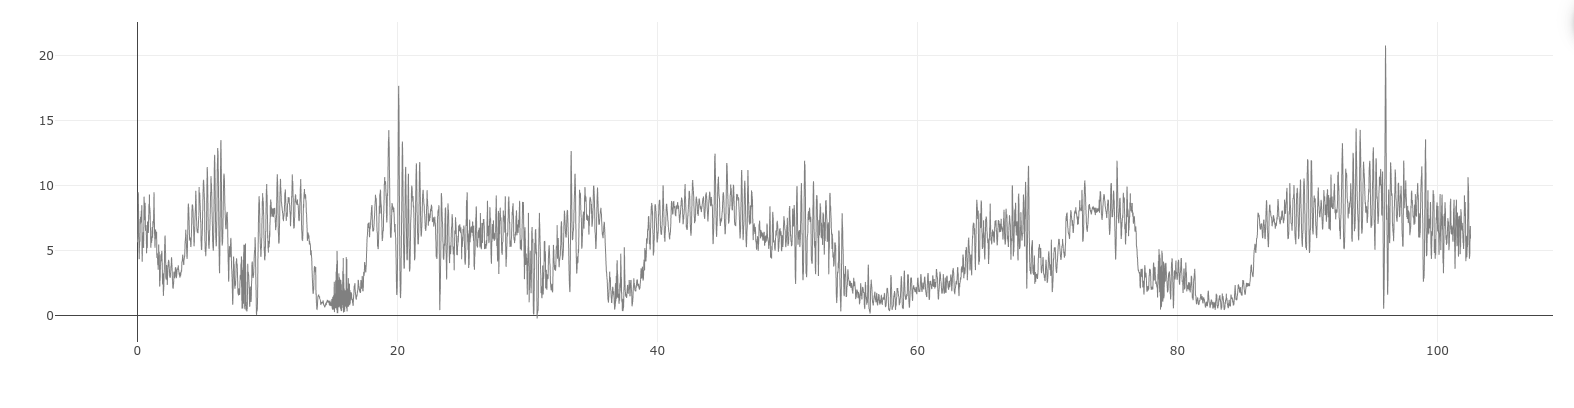
\includegraphics[width=\textwidth]{gfx/Zeitreihe_before.png} 
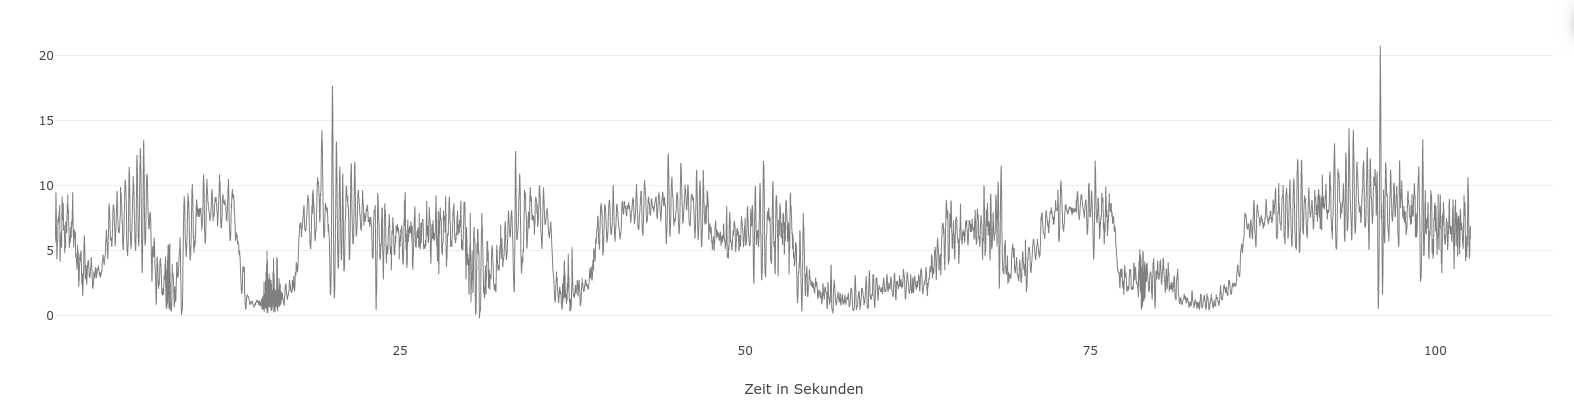
\includegraphics[width=\textwidth]{gfx/Zeitreihe_after.png}
\caption{Zeitreihe vor und nach dem Ordnungschaffen}
\label{fig:timeSeries_Before_After}
\end{figure}
\noindent
Der Defaultlinegraph von plotly.js ist in Abbildung \ref{fig:timeSeries_Before_After} zu sehen. Um Ordnung zu schaffen, wird die Nulllinie entfärbt sowie die x-Achse auf null fixiert. Es handelt sich um eine Zeitreihe, und es gibt keine negative Zeit in diesem Anwendungsfall, da die Messung immer bei null Sekunden startet. Bei der y-Achse wird die Null entfernt, da sich die beiden Nullen von der x- und y-Achse sonst überschneiden würden. Dazu werden die Ticks auf der x-Achse auf vier Stück pro Graph begrenzt, die sich automatisch berechnen. Auch die hellen Linien im Hintergrund der Ticks aus der x-Achse werden entfernt. Zudem wird bei der Hoverfunktion des Graphen für Ordnung gesorgt. Das Label hat eine dezentere Hintergrundfarbe und die Werte, die im Label dargestellt werden, werden gerundet. Diese Änderung ist in Abbildung \ref{fig:timeSeries_label_Before_After} zu sehen. 
Auch der Graph nach dem Ordnungschaffen ist in Abbildung \ref{fig:timeSeries_Before_After} zu betrachten.\\\\
\begin{figure}[h!]
\centering
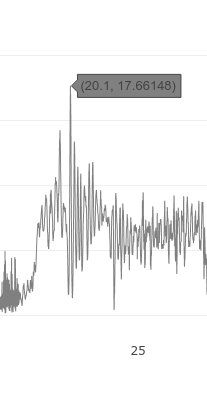
\includegraphics[width=0.15\textwidth]{gfx/Zeitreihe_label_before.png} 
\hspace*{+2cm}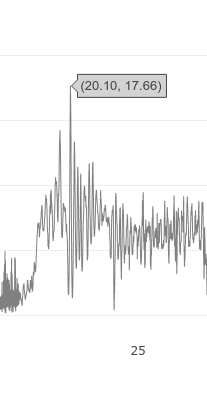
\includegraphics[width=0.15\textwidth]{gfx/Zeitreihe_label_after.png}
\caption{Hoverlabel der Zeitreihe vorher und nachher}
\label{fig:timeSeries_label_Before_After}
\end{figure}
\noindent
4. Aufmerksamkeit bündeln:\\
Bei den Zeitreihen gibt es, in Bezug auf den Punkt „Aufmerksamkeit bündeln“, einen Sonderfall, da die Trenderkennung von Anfang an genutzt werden kann. Die Minima und Maxima sind bei den Zeitreihen am interessantesten für die Benutzer, also bietet es sich an, diese direkt am Anfang anzuzeigen und die anderen Komponenten der Trenderkennung optional einbindbar zu gestalten. Durch das Markieren der Minima und Maxima wird die Aufmerksamkeit des Benutzers unmittelbar auf die wichtigen Punkte gelenkt. Zusätzlich lassen sich per Seitenmenü die anderen Trenderkennungsteile aktivieren und für den Nutzer dynamisch ändern. Bei den Minima und Maxima werden, wie bereits in der Trenderkennung, die Markerfarben und -größen geändert, damit sie herausstechen. Allerdings reicht es, für beide jeweils die gleiche Farbe zu nutzen, da durch die Ausrichtung der markierten Punkte klar wird, was ein Minimum und was ein Maximum ist. Auch bietet es sich an, die Drifterkennung direkt erkennbar zu machen, ohne dass der Benutzer diese händisch aktivieren müsste. \\\\
5. Geschichte erzählen:\\
Die Geschichte dieses Graphen wird mit der Trenderkennung erzählt. Wo sind Minima und Maxima, wo tritt ein Drift oder Offset auf, welche Werte springen über den Wertebereich -- all diese Fragen werden mit der Trenderkennung geklärt und für den Benutzer dargestellt. Wichtig ist dabei, dass die Trenderkennung dynamisch bleibt, da je nach Zeitreihe und je nach Bauteil unterschiedliche Maxima und Minima auftreten können. Dazu wird ein Seitenmenü erstellt, das die verschiedenen Teile der Trenderkennung aktivierbar sowie dynamisch einstellbar macht. Beispielhaft wird das Seitenmenü mit dynamischer Anpassung in Abbildung  \ref{fig:zeitreihe_mit_trenderkennung} dargestellt.
\begin{figure}[h!]
    \centering
    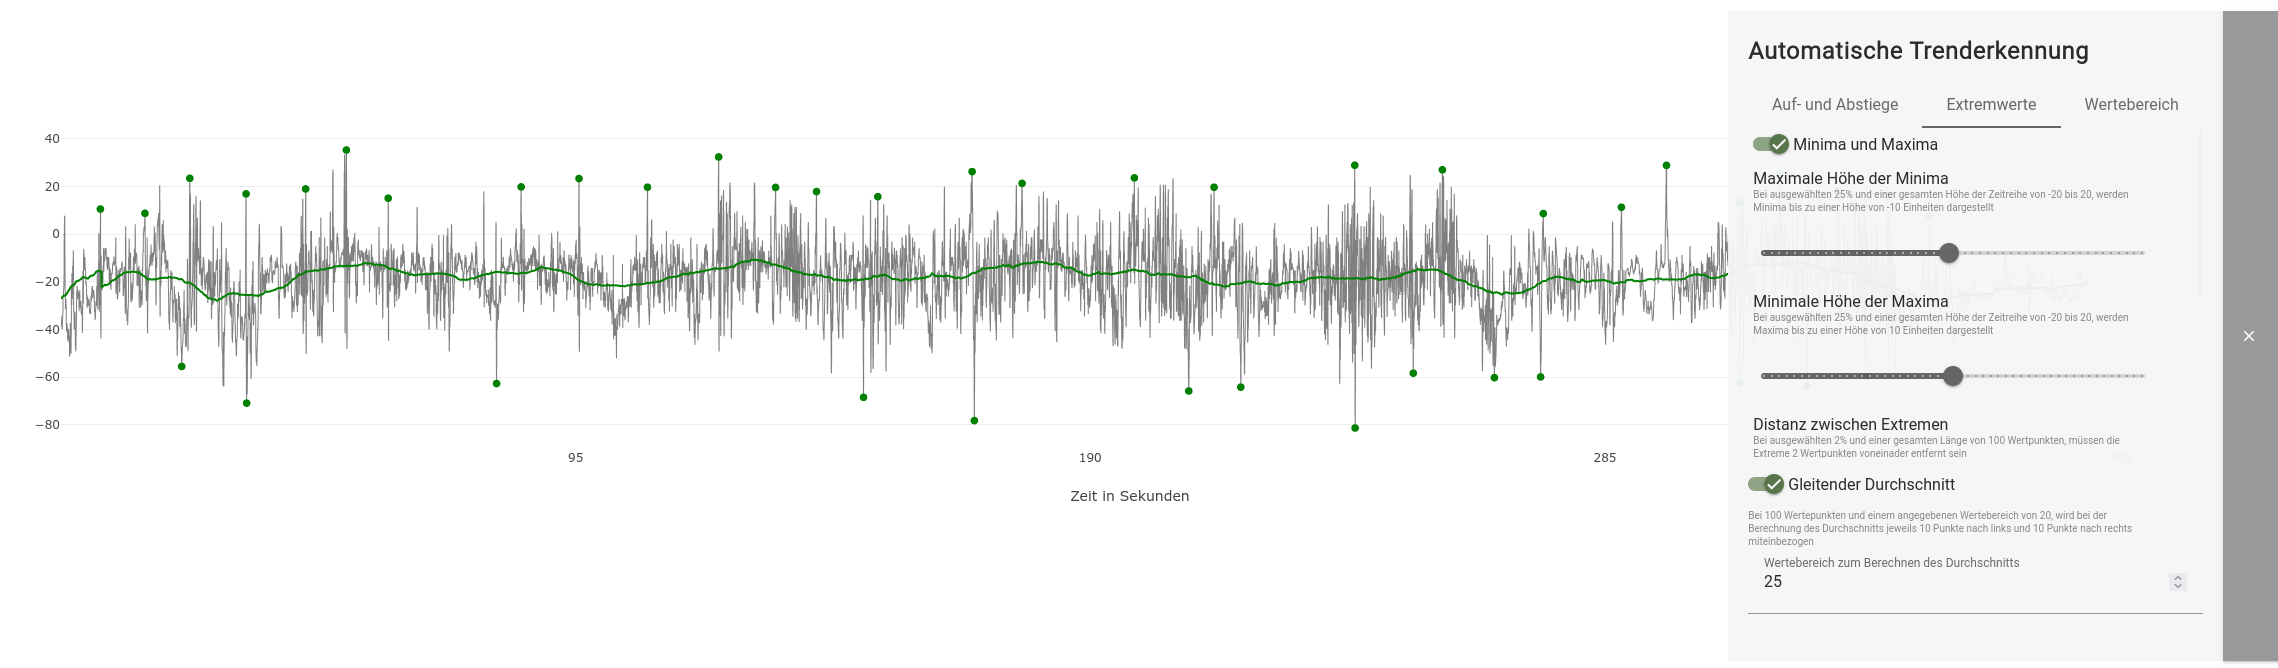
\includegraphics[width=\linewidth]{gfx/zeitreihe_mit_trenderkennung.png}
    \caption{Zeitreihe mit Trenderkennungsmenü sowie dynamisch eingestelltem gleitendem Durchschnitt}
    \label{fig:zeitreihe_mit_trenderkennung}
\end{figure}
\chapter{Implementation der Webseite}
Webseiten sind einfach zu erreichen, da für die Verwendung nur ein Browser benötigt wird. Daher fiel bei diesem Projekt die Wahl auf eine Implementation mittels Webseite. Die Webseite wird mit Angular entwickelt. Wie bereits erwähnt, gibt es bereits ein Monorepository, das auf Angular Material aufbaut. Für die Implementation von dem Monorepository wurde Nx verwendet \cite{Nx.}.  Angular Material ist eine Komponenten-Bibliothek, die verschiedene visuelle Komponenten bereitstellt, wie Buttons, Form-Fields mit verschiedenen Eingabemöglichkeiten und Slider. Da die Bibliothek von den Angular-Entwicklern selbst implementiert wurde, sind alle Komponenten bereits getestet und lassen sich ohne Probleme integrieren und erweitern \cite{Angular.2024}. Angular  basiert auf einem Komponentensystem. Das bedeutet, Angular wird aus verschiedenen Komponenten zusammengesetzt, die alle eigenes HTML, TypeScript und eigenen CSS-Code haben. Also können Komponenten beliebig oft verwendet werden und sind in ihrer Funktionalität trotzdem geschlossen. In dem bestehenden Monorepository gibt es verschiedene geteilte Komponenten, beispielsweise einen App-Core, der für alle Apps die Navigation und das Routing implementiert, Fehlerbehandlung, Authentifizierung und verschiedene visuelle Komponenten, die auch in dieser Webseite verwendet werden. Zu den visuellen Komponenten zählen:
\begin{multicols}{3}
    \begin{itemize}
        \item Buttons
        \item Cards
        \item Charts 
        \item Dynamic Dialog
        \item Loading Indicator
        \item Table
        \item Map
        \item Warning
        \item Error Stacker
    \end{itemize}
\end{multicols}
\noindent
Die geteilten Komponenten nutzen, genau wie die Angular-Material-Komponenten, Farbpaletten, die jeweils eine primäre, eine Akzent-, eine Warn- und eine Success-Farbe zugewiesen bekommen. Auf der Primärfarbe basieren die verschiedenen grünen Farbtöne, die in den Data-Storytelling-Graphen verwendet wurden. Dazu wurde das Tool coolors \cite{FabrizioBianchi.} genutzt, um jeweils hellere und dunklere Töne basierend auf der Farbe zu erzeugen.
\begin{figure}[h!]
\centering
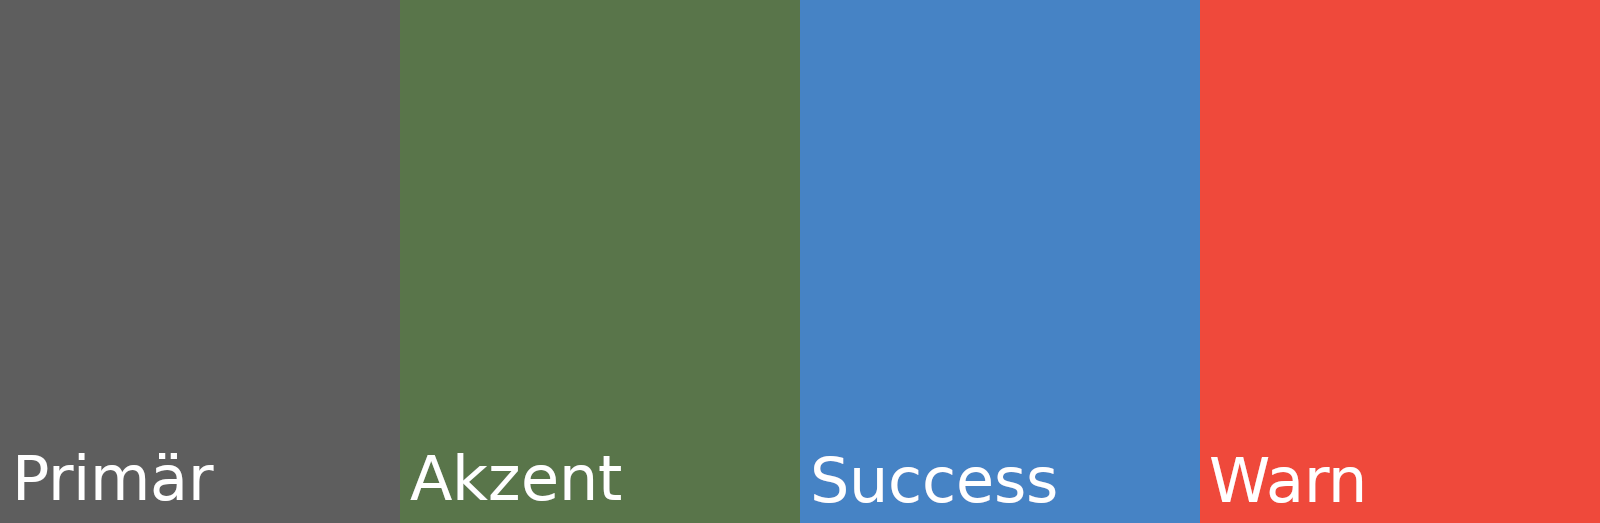
\includegraphics[scale=0.6]{gfx/palette.png}
\caption{Farbpalette für die Webseite}
\label{fig:palette}
\end{figure}
\\\\Die App-Core-Komponente, die die Webseite auch nutzt, generiert die Navigation für die App automatisch aus einer JSON-Datei und transformiert die Navigation, je nachdem welche Unterseite aufgerufen ist. Die Navigation, die in der JSON-Datei festgelegt wird, entspricht dem Datentyp \texttt{NavigationItem} aus \ref{appendix:dataset_types}. Über die Komponente wird auch das Ein- und Ausloggen durchgeführt. Für das User-Management wird Keycloak verwendet \cite{KeycloakAuthorsTheLinuxFoundation.2023}. Die Navigationskomponente übernimmt auch das Routing für die Unterseiten. Diese werden als einfache Bibliotheken mit eigenen Komponenten und Services angelegt. Zusätzlich gibt es einen automatischen Ladebalken, der jedes Mal, wenn eine Aktion mit dem Netzwerk ausgeführt wird, eingeblendet wird. Der Ladebalken kann anhand von einem Tutorial implementiert werden \cite{KeithStrickland.2020} und die Navigation ist ähnlich einem vorhandenen Beispiel \cite{sahilshah.2023}.
\\\\ 
Allgemein gibt es für Angular gute Tutorials, bei der Entwicklung der Webseite wurde unter anderem auf die Anleitungen von \cite{Angular.2022} für die allgemeine Implementation, \cite{DavidAkim.2022} für die Benutzung von plotly.js mit Angular und \cite{JonathanCardoso.2021} für die Verwendung von generics in Typescript zurückgegriffen.
\section{Implementation API und State}
Die Implementation der API wurde durch die bereits existierende Monorepository-Struktur und durch die Verwendung von @NgRx/data \cite{NgRx.io.2024} deutlich vereinfacht. Ohne diese Erweiterung muss für jede Schnittstelle ein Service angelegt werden, der die Anfragen steuert. Mit @NgRx/data und einem generischen Services wird diese Arbeit zumindest für die CRUD-Anfragen (Create, Read, Update und Delete) abgenommen. Die Erstellung eines generischen Datenservice zum Abwickeln der CRUD-Anfragen wird in folgendem Tutorial beschrieben: \cite{A.Waris.2023}.
Dieser generische Datenservice vererbt mithilfe von dem Keyword \texttt{extends} an die einzelnen Entitätenservices, die von @NgRx/data erstellt wurden, und somit können die bereits vorhandenen CRUD-Funktionen in Sonderfällen pro Entität angepasst werden \cite{MicrosoftTypeScript.2024}.  
Zudem wurde bei der Erstellung des Monorepositorys darauf geachtet, die Datentypen möglichst wiederzuverwenden, deshalb können viele Services genutzt werden, die bereits existieren.\\
Eine Besonderheit von NgRx ist die Bereitstellung einer Funktionalität mit Namen Store, dabei wird lokales State-Management für Angular-Apps bereitgestellt \cite{NgRx.io.2024b}. Es wird nicht nur für jede Unterseite ein eigener State erstellt, der Informationen Unterseiten übergreifend bereitstellen kann, sondern auch der Zugriff auf die Daten erleichtert, die von den API-Anfragen zurückgegeben werden. Dadurch kann es Usern ermöglicht werden, auch nach dem Navigieren auf der Seite wieder zu ihren ausgewählten Analysen zurückzukommen. NgRx benutzt verschiedene Komponenten, um das State-Management zu ermöglichen. In der folgenden Abbildung \ref{fig:NgRx} von \cite{NgRx.io.2024b} werden die verschiedenen Komponenten sowie ihr Zusammenspiel dargestellt.
\begin{figure}[!h]
    \centering
    \includegraphics[width=0.75\linewidth]{gfx/NgRx.png}
    \caption{NgRx-Flow und -Komponenten \cite{NgRx.io.2024b}}
    \label{fig:NgRx}
\end{figure}
Die Komponenten sind:
\begin{description}
    \item[selector]\hfill \\
    Die Selektoren sind dazu da, die Daten im Store für die Benutzung in den Angular-Komponenten bereitzustellen. Dabei können die Daten umgeformt oder gefiltert werden.
    \item[component]\hfill \\
    Die Angular-Komponente, die für die Darstellung der gelieferten Daten zuständig ist. Durch Benutzereingaben können Actions getriggert werden.
    \item[action]\hfill \\
    Actions sind dazu da, entweder Daten von den Benutzereingaben in den Store zu schreiben oder Effekte zu triggern. 
    \item[effects]\hfill \\
    Effekte sind für die Kommunikation mit den von @NgRx/data erstellten Services vorgesehen. Sie starten die API-Anfragen und können die Ergebnisse verwalten. Außerdem können die Effekte erneut Actions abschicken, um beispielsweise Fehlermeldungen oder Anfragen, die von anderen Anfragen abhängen, zu starten.
    \item[service]\hfill \\
    Die Services werden mit @NgRx/data erstellt und können beliebig für weitere Anfragen außerhalb von CRUD erweitert werden.
    \item[reducer]\hfill \\
    Reducer ermöglichen den Zugriff auf den Store, sowohl um die Variablen zu ändern als auch um diese zu lesen. 
    \item[store]\hfill \\
    Die bereits angefragten Daten werden hier zwischengespeichert und für jeden Selector in der App abrufbar gemacht.
\end{description}
In dem genutzten Monorepository wurde ein generischer State erstellt, der mithilfe von allgemeinen Reducern und Actions einiges an Schreibarbeit erspart. Es müssen pro Unterseite Selektoren und Effects angelegt werden. Die allgemeinen Actions basieren auf einem \texttt{ACTION\_TYPE} enum, der beispielsweise für die Selektion der zu analysierenden Daten zuständig ist. Dabei werden der \texttt{ACTION\_TYPE} für die passende Auswahl sowie die ausgewählten IDs an den State weitergegeben. Einige Beispiele, wie der \texttt{ACTION\_TYPE} enum formuliert werden kann, befinden sich in \ref{appendix:dataset_types}. 
\section{Implementation Seiten}
Im Laufe der Entwicklung wurden zusätzlich zu den bereits bekannten Seiten aus den Interviews noch weitere Seiten festgelegt. Somit werden für die Webseite die folgenden Unterseiten erstellt:
\begin{itemize}
    \item Datenbasis
    \item Alternativer Kilometerzähler
    \item Fingerprints
    \item Überwachung Dauerlauferprobung
    \item Vergleich von Einsatzdaten
\end{itemize}
Die Datenbasis wird mithilfe eines Generic Service implementiert, der übergreifend über das Monorepository alle Datenbasen erstellt. Allerdings wird in diesem Anwendungsfall das Diagramm aus \ref{section:Prozentuale_Schädigung} hinzugefügt. Dabei werden der State oder auch die API-Aufrufe von einem Base-Service geregelt. Dadurch müssen nur die geteilten Komponenten für die Datenbasis im HTML eingebunden werden. Dazu  zählen eine Komponente für die Karte, die die Einsatzorte darstellt, das hervorgehobene Rechteck neben der Karte, das die zusätzlichen Informationen zu den ausgewählten Daten zeigt, und die einzelnen Karten pro Fahrzeug. Über dieses Template wird der Graph hinzugefügt, der für jedes Fahrzeug die passenden Daten darstellt. Dazu hat die Datenbasis das Attribut „selected Vehicle“, um die passenden Daten sowohl für die zusätzlichen Informationen als auch für den Graphen zu filtern.\\\\ Der alternative Kilometerzähler wurde aufgrund der Entwicklung des Diagrammes aus \ref{section:Prozentuale_Schädigung} hinzugefügt, da es praktisch ist, alle Fahrzeuge und deren aktuelle Schädigungen auf einen Blick zu sehen. Durch einen generischen Datenservice, der die API-Aufrufe für alle Fahrzeuge regelt, lassen sich die vorhandenen Fahrzeuge über den State abfragen und in eine eigene Komponente geben, die die Darstellung pro Fahrzeug regelt. Hierfür wird der gleiche Service verwendet, der auch in der Datenbasis die Graphen bereitstellt.\\\\ Die Fingerprints sind zur alleinigen Darstellung des Diagramms für die Fingerprints da. Da es sich bei den Fingerprints um eines der wichtigsten Werkzeuge für diesen Anwendungsfall handelt, wurde die Unterseite hinzugefügt. Der State wird vom generisch implementierten State geregelt. Dabei müssen nur die Selektoren und Effekte hinzugefügt werden, die Actions und der Reducer sind für jede Seite gleich, die mit dem generischen State erstellt wurde. Da für die Seite nur die Fingerprints in der aktuellen Auswahl relevant sind und die Auswahl vom generischen State geregelt wird, wird lediglich ein Effekt mit der Anfrage an das Backend bezüglich der ausgewählten Fingerprints benötigt.\\\\
Die Dauerlauferprobung setzt sich aus den Diagrammen der Dauerlauferprobung (\ref{section:dauerlauferprobung}), des Fahrzeugbildes mit den eingefärbten Teilen (\ref{sec:vehicle-images)} und einer Tabelle mit weiteren Informationen zur Erprobung zusammen. Danach kann der Benutzer über den Graphen der Erprobung einen Punkt in der Erprobung auswählen. Über diese Auswahl wird der Graph mit der kumulierten Schädigung (\ref{section:schaedigung}) befüllt. Über diesen Graphen kann wiederum eine einzelne Messung ausgewählt werden, die dann als Zeitreihe \ref{sec:timeseries} angezeigt werden kann. Dadurch können alle relevanten Daten für die Dauerlauferprobung angezeigt werden. Alternativ kann je nach den Bedürfnissen auch nur ein grober Überblick über die vorhandenen Messungen erfasst werden. Auch der State auf dieser Seite wird vom generischen State geregelt. Durch die vielen verschiedenen Daten, die angefragt oder angezeigt werden können, werden mehrere \texttt{ACTION\_TYPES} für jede einzelne Benutzerinteraktion benötigt.\\\\
Die Seite zum Vergleich der Einsatzdaten stellt mehrere Daten gleichzeitig dar. Zunächst werden der Graph mit den Fahrzeugbildern und die gleiche Tabelle wie in der Dauerlauferprobung dargestellt. Um einen Vergleich über die Daten zu gewährleisten, wird der Graph mit der kumulierten Schädigung (\ref{section:schaedigung}) genutzt. Über die Auswahl des Benutzers können die einzelnen Messungen als Zeitreihen (\ref{sec:timeseries}) dargestellt werden. Zudem gibt es eine Darstellung, die die einzelnen Kollektive zeigt. Sie wurde in dieser Arbeit nicht mit Data-Storytelling überarbeitet, da Kollektive eine feste Größe im Feld der Betriebsfestigkeit \cite{Gotz.2020} sind. Bei den Kollektiven werden laut \cite{PatrickPfeiffer.17.10.2022} lediglich die höchsten Ausschläge des Messsignals betrachtet. Da es bei der Darstellung der Kollektive nicht möglich ist, einen Handlungsaufruf zu starten oder sonstige Points of Interest hervorzuheben, eignet sich diese Darstellungsart nicht für das Data-Storytelling. Der State der Vergleich von Einsatzdatenseite wird vom generischen State abgewickelt. Die API für die Fingerprints und die Dauerlauferprobung sind vor Fertigstellung dieser Masterarbeit noch nicht fertig implementiert, weswegen auf der Webseite aktuell für beide ein Beispieldatensatz im passenden Format bereitgestellt wird.\\\\
Alle Unterseiten sind gleich aufgebaut. Zuerst wird eine Containerkomponente implementiert, die die Verteilung der Daten an die Unterkomponenten regelt. Im HTML dieser Komponente wird der Seitenaufbau erstellt und es werden die Unterkomponenten angesprochen. Die einzelnen Unterkomponenten sprechen die passenden Services an, um die Visualisierungen zu erstellen. Die Daten, die in den Services weiterverarbeitet werden, werden an verschiedene Komponenten weitergeleitet, um die Daten darzustellen, beispielsweise die Shared-Chart- oder die Shared-Tabellen-Komponenten. Da sich auf den Seiten einige Diagramme und Visualisierungen wiederholen, bietet es sich an, diese in eigene Komponenten auszulagern, beispielsweise die Fingerprints oder die Fahrzeugvisualisierung mit den Bildern und Image-Maps. Dadurch lässt sich vermeiden, dass sich Codestücke wiederholen. Auch die Komponente zur Auswahl der Fahrzeuge wird einmal implementiert und dann mithilfe des Komponentensystems auf mehreren Seiten genutzt. Die Auswahl hat einen Toggle, über den entschieden werden kann, ob die Auswahl für Einzelfahrzeuge oder für Fahrzeugtypen gelten soll. Anhand dieser Auswahl wird eine JSON-Konfiguration erstellt und die Auswahl dynamisch erzeugt. Die JSON-Konfiguration wird mittels des Datentyps \texttt{DynamicDataSelectData} in \ref{appendix:dataset_types} erstellt. Dadurch können beliebig viele Auswahlfelder, eine Warnung oder ein Button konfiguriert werden. Jedes Auswahlfeld wird mit dem Typ \texttt{DynamicDataSelectControls} erstellt. Dabei ist insbesondere das Feld \texttt{influences} interessant, da dadurch Beziehungen zwischen den Feldern ausgewiesen werden können. Für zusätzliche Validierungen können die Typen \texttt{DynamicFormValidatorConfig} oder \texttt{DynamicFormAdditionalConfig} genutzt werden, beispielsweise kann hier auch die Optionalität der Felder konfiguriert werden.
\section{Implementation Graphen}
Die Graphen werden mit plotly.js für Angular implementiert. Grundsätzlich setzen sich die Charts aus Layout und Traces zusammen, in \ref{appendix:graph_types} ist das passende Interface \texttt{Chart} zu sehen. Das Layout ist für die visuelle Darstellung des gesamten Graphen verantwortlich, während die Traces die einzelnen Wertedarstellungen bilden. Generell gibt es bei plotly.js mehrere Wege, um Informationen zusätzlich zu den x- und y-Werten anzuzeigen. Laut der plotly.js-Dokumentation \cite{Plotly.2024b} gibt es sowohl Annotations als auch Shapes, um die Graphen zu erweitern.\\\\ Bei der Erstellung der Graphen wird pro Graph ein Service erstellt, der die Daten auswertet und wenn nötig transformiert sowie das Layout bildet und an die Chart-Komponente weitergibt. Um beispielsweise den Zeitreihen-Graphen darzustellen, wird ein Layout mit den folgenden Parametern erstellt:
\begin{lstlisting}[language=Typescript]
    {
      showlegend: false,
      annotations: this.createAnnotations(testData.values, trends),
      shapes: this.createShapesForRisesAndFalls(time, trends),
      hoverlabel: { bgcolor: 'lightgray' },
      xaxis: {
        zeroline: false,
        rangemode: 'tozero',
        autorange: true,
        tickvals: tickvals.map((val) => val * tickSteps),
        ticktext: [''].concat(
          tickvals.slice(1).map((val) => (val * tickSteps).toString())
        ),
        title: { text: 'Zeit in Sekunden' },
        showgrid: false,
        hoverformat: '.2f',
      },
      yaxis: {
        zeroline: false,
        autorange: true,
        hoverformat: '.2f',
      },
    };
\end{lstlisting}
Die Annotations und Shapes werden von einer separaten Funktion mit den nötigen Werten für die Trenderkennung gefüllt. Der Parameter \texttt{showlegend} konfiguriert, ob die Legende dargestellt werden soll, in der die verschiedenen Traces angezeigt werden. Durch den Parameter \texttt{hoverlabel} kann das Hoverlabel mit verschiedenen Variablen angepasst werden, wie in diesem Beispiel der Hintergrundfarbe. Andere Anpassungsmöglichkeiten sind die Farbe, Schriftart, ob noch zusätzliche Informationen im Hoverlabel angezeigt werden sollen und verschiedene Formatierungsmöglichkeiten für diese Informationen. Es lassen sich sowohl die x- als auch die y-Achse genau anpassen. Bei dem Layout für die Zeitreihen ist besonders interessant, dass durch die Überschneidung des Nullpunktes auf beiden Achsen zweimal die Null angezeigt wurde. Aufgrund der Reduzierung des Visual Clutters beim Data-Storytelling wird durch die Funktion, die im Layout in der x-Achse die \texttt{tickvals} und den \texttt{ticktext} berechnet, die Null auf der x-Achse durch einen leeren String ersetzt. Das reduziert die Darstellung um eine Null für den Punkt an den sich die beiden Achsen schneiden, anstatt zwei Nullen nebeneinander darzustellen. Die \texttt{tickvals} legen fest, wo auf der Achse ein Tick gesetzt werden soll. Dieser Wert wird durch eine einfache Berechnung ermittelt, die die Dauer der Zeitreihe durch vier teilt und das Ergebnis dann rundet, um auf eine sinnvolle Zahl zu kommen. Dadurch werden immer vier Ticks dargestellt. Die Parameter \texttt{zeroline} und \texttt{showgrid} sind beide für die Darstellung des Grids zuständig, wobei \texttt{zeroline} die Nulllinie hervorhebt und \texttt{showgrid} das Grid vollständig ausblendet. Das Attribut \texttt{rangemode} gibt an, welcher Art die Beschränkungen des Grids sind: Bei \texttt{tozero} ist die Nulllinie die untere Grenze des Grids, bei \texttt{auto} wird das Grid passend zu den Graphen skaliert. Das \texttt{hoverformat} schränkt die Formatierung im Hoverlabel auf zwei Stellen hinter dem Komma ein.\\ Für die Erstellung der Wertedarstellungen wird ebenfalls ein Objekt definiert. Dieses ist im Folgenden am Beispiel der Zeitreihen abgebildet:
\begin{lstlisting}[language=Typescript]
    {
        x: this.calculateTimeForFrequency(
          testData.frequency,
          testData.values.length
        ),
        y: testData.values,
        hoverinfo: 'name +x+y',
        type: 'scattergl',
        mode: 'lines+markers',
        marker: {
          color: this.getColorForMarkers(
            trends?.maximaAndMinima,
            testData.values
          ),
          size: 8,
        },
        line: {
          color: 'gray',
          width: 1,
        },
        name: 'Zeitreihe',
    },
\end{lstlisting}
Es werden zunächst zwei Arrays mit den jeweiligen x- und y-Werten festgelegt. Anschließend folgt die Zusammensetzung der Daten, die im Hoverlabel dargestellt werden. Als \texttt{type} wird der Typ der Wertedarstellung definiert, der Default-Wert ist meist \texttt{scatter}. Weil aber besonders bei der Trenderkennung die Implementation der Darstellungen und Rechnungen aufwendiger war, was zu Performanceeinbußen führte, wenn der Graph als klassisches SVG implementiert wurde, wurde der Typ \texttt{scattergl} gewählt. Dadurch hat plotly.js die Möglichkeit, die Graphen auch mit WebGL rendern zu lassen. WebGL ist laut \cite{MDNcontributors.2024b} eine JavaScript-API, die mithilfe von OpenGL in der Lage ist, die Hardware des Computers durch den Browser anzusteuern, und dadurch die Zeit für das Rendern des Graphen deutlich minimieren kann \cite{Plotly.2024b}. Durch den \texttt{mode} lässt sich die Darstellung der Werte als Linien, Marker oder beides anwenden. Zuletzt können die Marker und die Linien jeweils mit Farben und Größen visuell angepasst werden. Mit dem Parameter \texttt{name} wird der Name festgelegt, der beispielsweise in der Legende verwendet wird. 
Durch diese Vorgehensweise können mit plotly.js alle in dieser Arbeit erstellten Graphen implementiert werden.
